\documentclass{article}
\usepackage{amsfonts,amssymb,amsmath,amsthm,mathtools,bm}
\numberwithin{equation}{section}
\usepackage{booktabs}
\usepackage{array,tabularx}
\usepackage{enumitem}
\setlist[itemize]{noitemsep,topsep=2pt}
\usepackage[margin=1in]{geometry}
\usepackage[numbers]{natbib}
\usepackage{authblk}
\usepackage[ruled,linesnumbered]{algorithm2e}
\usepackage{xcolor}
\definecolor{purple}{rgb}{0.50,0.00,0.50}
\usepackage[colorlinks,citecolor=purple,linkcolor=blue]{hyperref}
\usepackage[nameinlink]{cleveref}

\renewcommand{\baselinestretch}{1.15}

\newtheorem{theorem}{Theorem}[section]
\newtheorem{corollary}{Corollary}[section]
\newtheorem{lemma}{Lemma}[section]
\newtheorem{proposition}{Proposition}[section]
\newtheorem{definition}{Definition}[section]
\newtheorem{remark}{Remark}[section]
\newtheorem{assumption}{Assumption}[section]

\crefname{assumption}{Assumption}{Assumptions}
\Crefname{assumption}{Assumption}{Assumptions}
\crefname{algorithm}{Algorithm}{Algorithms}
\Crefname{algorithm}{Algorithm}{Algorithms}

\newcommand{\R}{\mathbb{R}}

\usepackage{graphicx}
\newtheorem{fact}{Fact}[section]
\crefname{fact}{Fact}{Facts}
\Crefname{fact}{Fact}{Facts}

\title{Parameter-Free Universal Trust-Region Methods\\
for Nonconvex--Strongly-Concave Minimax Optimization}
\author{}
\date{}

\begin{document}
\maketitle

% \begin{abstract}
% We study second-order stationarity for smooth nonconvex--strongly-concave
% minimax problems without supplying any smoothness or strong-concavity
% parameter to the algorithm.  Our method combines a gradient-scaled
% universal trust-region model with persistent residual reduction by SCAR.
% A Newton correction makes the value-function gradient error quadratic
% in the inner distance, while a corrected value provides a proxy that can
% be tracked across accepted steps and scale changes.  A gradient-level
% potential controls outer progress, and its associated cubic-path bound
% amortizes the variable work needed to track the inner maximizers.
% Writing $\kappa=\ell/\mu$ for the inner condition number, $\rho$ for the
% joint Hessian-Lipschitz constant, and $\Delta_P$ for the initial
% value-function gap, the leading complexities are
% $O(\Delta_P\kappa^{3/2}\sqrt\rho\,\epsilon^{-3/2})$ trust-region
% subproblems and
% $O(\Delta_P\kappa^2\sqrt\rho\,\epsilon^{-3/2})$ inner-gradient
% evaluations.  All remaining costs are additive and at most cubic
% logarithmic in $1/\epsilon$ for each fixed instance.  Neither
% $\log(1/\epsilon)$ nor $\log\kappa$ multiplies the leading inner-work
% term.  The guarantee is class-uniform asymptotic: after fixing common
% regularity constants $(\ell,\mu,\rho)$, one positive accuracy threshold
% works for every payoff and initialization in that class.  The algorithm
% does not use these constants, but it does not certify that a requested
% accuracy lies below this unknown threshold.  Parameter-free
% unconstrained UTR and the SCAR guarantees are presented as preliminary
% tools, with their supporting analysis deferred to the appendix.
% \end{abstract}

\section{Introduction}
\label{sec:introduction}

We consider smooth nonconvex--strongly-concave (NC--SC) minimax
optimization
\begin{equation}\label{eq:minimax-intro}
 \min_{x\in\R^{d_x}}\max_{y\in\R^{d_y}}f(x,y),
\end{equation}
where $f(x,\cdot)$ is strongly concave for every $x$, while
$f(\cdot,y)$ may be nonconvex. Strong concavity makes the inner
maximizer $y^*(x):=\arg\max_y f(x,y)$ well defined and gives rise to
the primal function $P(x):=\max_y f(x,y)$.
Under standard smoothness assumptions, $P$ is twice differentiable
but generally nonconvex. An approximate first-order stationary point
of $P$ therefore need not capture local optimality, which motivates
the search for approximate second-order stationary points.

Second-order algorithms for NC--SC minimax optimization have been
developed using cubic regularization, trust-region methods, and other
Newton-type updates
\citep{luo2022finding,chen2023cubic,yao2025trust,
wang2025gradient,chen2026hsda}.
A representative method is Minimax Cubic Newton (MCN)
\citep{luo2022finding}, which approximates the gradient and Hessian of
$P$ through inner maximization and achieves the characteristic
$O(\epsilon^{-3/2})$ second-order oracle complexity. Several subsequent
methods attain the same $\epsilon^{-3/2}$-type outer dependence under
related second-order stationarity criteria. More recently,
joint-minimization reformulations have led to methods that avoid
repeatedly solving the inner maximization
\citep{ma2026linesearch,ma2026singleloop}.

For methods that construct approximate derivatives of $P$ through
inner maximization, the outer iteration complexity alone does not
describe the total computational work. At each outer iterate $x_k$,
one must approximate $y^*(x_k)$ accurately enough that the resulting
first- and second-order information of $P$ can be used reliably.
In MCN, accelerated gradient ascent is used for this purpose.
Its first-order oracle complexity is stated in
$\widetilde O(\epsilon^{-3/2})$ form, and the explicit bound contains a
logarithmic dependence on the target accuracy multiplying the leading
outer-order term. 

Our method builds on the universal trust-region (UTR) framework of
\citet{jiang2026utr}. We first formulate a general inexact UTR
interface in which working queries provide approximate values,
gradients, and Hessians, and validation queries check possible
solutions. Its convergence theorem controls both the outer iteration
count and the cumulative path needed for inner-work analysis.
The minimax algorithm realizes this interface through corrected
primal-function oracles and persistent calls to SCAR
\citep{lan2026optimal}. It retains the inner solver's curvature
estimates across successive maximization problems and adjusts inner
accuracy to the current outer scale. This gives the desired leading
outer and inner complexity without supplying smoothness or
strong-concavity parameters to either component.

\subsection{Main Contributions}
\label{sec:contributions}

Our contributions concern the total inner work and the removal of
problem parameters from the executable minimax method. The existing
implicit gradient and Schur-complement Hessian are ingredients of
the construction.

\paragraph{Sharper total inner-gradient complexity.}
Let $\ell$ and $\rho$ denote the Lipschitz constants of the joint
gradient and Hessian of $f$, respectively, let $\mu>0$ be the
strong-concavity modulus of $f(x,\cdot)$, and set
\[
 \kappa:=\ell/\mu,\qquad
 \Delta_P:=P(x_0)-\inf_xP(x),\qquad
 M_P:=4\sqrt2\,\kappa^3\rho.
\]
\Cref{alg:gradient-scaled-scar} combines the implicit gradient and
Schur-complement Hessian with an adaptive UTR step and accesses inner
maximization through observable gradient residuals.
The key estimate is a cumulative cubic bound on the accepted outer
steps, which amortizes the logarithmic costs of successive
warm-started inner calls. Persistent SCAR also shares its curvature
calibration across the whole run.
For each fixed regularity class and sufficiently small $\epsilon$,
\Cref{thm:gradient-scaled-scar} gives
\begin{align*}
 Q&=O\!\left(\Delta_P\kappa^{3/2}\sqrt\rho\,
                   \epsilon^{-3/2}\right)
       +O_{\rm fixed}(\log^3(e/\epsilon)),\\
 N_y&=O\!\left(\Delta_P\kappa^2\sqrt\rho\,
                   \epsilon^{-3/2}\right)
       +O_{\rm fixed}(\sqrt\kappa\,\log^3(e/\epsilon)),
\end{align*}
where $Q$ counts trust-region subproblems and $N_y$ counts all
inner-gradient evaluations. Here $O_{\rm fixed}$ permits constants
depending on the fixed payoff, regularity constants, and
initialization, but not on $\epsilon$.
Neither $\log(1/\epsilon)$ nor $\log\kappa$ multiplies the displayed
leading inner term. In particular, this removes the leading
target-accuracy logarithm in the explicit inner-gradient bound of
MCN. As a technical tool, \Cref{thm:total-complexity} gives a general
inexact UTR complexity bound, supplemented by the path estimates in
\Cref{prop:utr-budgets}; the minimax analysis invokes these results
after verifying the corrected-oracle error bounds.

\paragraph{A fully parameter-free second-order method.}
\Cref{alg:gradient-scaled-scar} uses only the initialization, target
tolerance, and universal numerical constants. Neither the outer
scheme nor SCAR requires $\ell$, $\mu$, $\rho$, $\kappa$, or $M_P$ as
an input. Working inner accuracy is restored through a number of
residual halvings determined by the observed outer step and current
scale; more accurate validation is reserved for candidate solutions.
The output satisfies
\[
 \|\nabla P(x_{\rm out})\|<\epsilon,\qquad
 \lambda_{\min}(\nabla^2P(x_{\rm out}))
 \ge-\frac{85}{16\sqrt6}\sqrt{M_P\epsilon}.
\]
A universal constant rescaling of the internal tolerance gives the
standard $\epsilon$-second-order guarantee defined in
\Cref{def:stationarity}.
The guarantee is class-uniform asymptotic: after fixing common
$(\ell,\mu,\rho)$, one threshold $\epsilon_0(\ell,\mu,\rho)>0$
works for every admissible payoff and initialization.
The algorithm does not know this threshold or certify that the
requested accuracy lies below it.
\Cref{sec:parameter-free-scope} explains this qualification through
the residual-only obstruction and the role of validation.

% !TeX root = ../revised_main.tex
\begin{table}[t]
\centering
\caption{Complexity comparison of deterministic second-order methods
for smooth NC--SC minimax optimization. Initial optimality gaps and
universal numerical constants are suppressed. For cited methods,
regularity-parameter dependence is shown when reported in a directly
comparable form; entries without such factors report only dependence
on $\epsilon$. For our method the
entries are leading terms, valid in the class-uniform small-accuracy
regime of \Cref{thm:gradient-scaled-scar}.}
\label{tab:ncsc-complexity}
\small
\renewcommand{\arraystretch}{1.18}
\setlength{\tabcolsep}{3pt}
\begin{tabularx}{\textwidth}{@{}
 >{\raggedright\arraybackslash}X
 >{\centering\arraybackslash}p{0.24\textwidth}
 >{\centering\arraybackslash}p{0.31\textwidth}
 >{\centering\arraybackslash}p{0.11\textwidth}@{}}
\toprule
Method & Outer complexity
 & \shortstack[c]{Total inner-gradient\\evaluations}
 & \shortstack[c]{Parameter-\\free}\\
\midrule
MCN \citep{luo2022finding}
 & $O(\kappa^{3/2}\sqrt\rho\,\epsilon^{-3/2})$
 & $\widetilde O(\kappa^2\sqrt\rho\,\epsilon^{-3/2})$
 & No\\[1mm]
MINIMAX-TR / MINIMAX-TRACE\newline \citep{yao2025trust}
 & $O(\epsilon^{-3/2})$
 & Not reported & No\\[1mm]
GRTR / LMNegCur\newline \citep{wang2025gradient}
 & $\widetilde O(\kappa^{3/2}\sqrt\rho\,\epsilon^{-3/2})$
 & $\widetilde O(\kappa^2\sqrt\rho\,\epsilon^{-3/2})$
 & No\\[1mm]
HSDA / IHSDA\newline \citep{chen2026hsda}
 & $\widetilde O(\epsilon^{-3/2})$
 & Not reported & No\\
\midrule
\Cref{alg:gradient-scaled-scar} (ours)
 & $O(\kappa^{3/2}\sqrt\rho\,\epsilon^{-3/2})$
 & $O(\kappa^2\sqrt\rho\,\epsilon^{-3/2})$
 & Yes\\
\bottomrule
\end{tabularx}

\vspace{1mm}
\begin{minipage}{0.97\textwidth}
\footnotesize
Here $\kappa=\ell/\mu$ and $\rho$ is the Hessian-Lipschitz constant
of $f$. The notation $\widetilde O(\cdot)$ is retained when used
in the cited reference. \emph{Not reported} means that the cited work
does not state a separate comparable total inner-gradient bound.
The complete bounds for \Cref{alg:gradient-scaled-scar} include
additive $O_{\rm fixed}(\log^3(e/\epsilon))$ and
$O_{\rm fixed}(\sqrt\kappa\,\log^3(e/\epsilon))$ terms for the outer
and inner counts, respectively. Its executable steps use no problem
parameters; the accuracy threshold in its guarantee is unknown.
\end{minipage}
\end{table}


\Cref{tab:ncsc-complexity} compares methods whose stated second-order
guarantees and oracle counts match the quantities considered here.
Cubic-LocalMinimax \citep{chen2023cubic}, whose complexity is stated
using a different local-minimax stationarity measure, is discussed
below without reparameterizing it for the table.
The recent single-loop regularized Newton method of
\citet{ma2026singleloop} has no inner maximization loop of the form
measured by the table's third column.

\subsection{Related Work}
\label{sec:related-work}
\paragraph{Implicit differentiation and primal-function estimators.}
\citet{ablin2020superefficiency} analyze the implicit gradient
estimator for functions defined through optimization and establish
its quadratic error in Proposition~2.3.
In minimax optimization, \citet{zhang2020newton} use the corresponding
total gradient and Schur-complement Hessian; see their
equations~(1.1)--(1.2).
These estimators are ingredients of the present work.
Our contributions concern their integration into an inexact UTR
method, the accumulated inner-gradient complexity, and parameter-free
tracking across changing inner objectives.

\paragraph{First-order methods for NC--SC minimax optimization.}
First-order methods for NC--SC minimax problems have been studied
extensively. Representative approaches include gradient
descent-ascent, multi-step ascent, proximal schemes, and accelerated
methods
\citep{nouiehed2019solving,lin2020gradient,lin2020near}.
Their complexity for finding first-order stationary points of the
primal function has also been studied from both upper- and lower-bound
perspectives; see, for example, \citet{zhang2021complexity} and the
references therein. These results form the first-order counterpart to
the second-order stationarity problem considered in this paper.

\paragraph{Second-order methods for NC--SC minimax optimization.}
\citet{luo2022finding} proposed MCN, which alternates accelerated
gradient ascent for approximating $y^*(x)$ with a cubic-regularized
update based on approximate first- and second-order information of the
primal function. Its leading bounds are
$O(\Delta_P\kappa^{3/2}\sqrt\rho\,\epsilon^{-3/2})$ second-order
oracle evaluations and
$\widetilde O(\Delta_P\kappa^2\sqrt\rho\,\epsilon^{-3/2})$
first-order oracle evaluations.
\citet{chen2023cubic} proposed Cubic-LocalMinimax and developed
inexact and stochastic variants, using cubic regularization to obtain
global convergence toward local minimax points. Their complexity is
formulated using a different stationarity measure, so we do not
convert it to the accuracy parameterization used in
\Cref{tab:ncsc-complexity}.

Trust-region approaches were developed by \citet{yao2025trust}, who
proposed MINIMAX-TR and MINIMAX-TRACE.
\citet{wang2025gradient} subsequently proposed gradient-norm
regularized trust-region and Levenberg--Marquardt methods, together
with inexact variants, and established
$\widetilde O(\kappa^{3/2}\sqrt\rho\,\epsilon^{-3/2})$ outer
complexity and
$\widetilde O(\kappa^2\sqrt\rho\,\epsilon^{-3/2})$ total
gradient-ascent complexity, suppressing the initial-gap dependence.
More recently, \citet{chen2026hsda} proposed homogeneous second-order
descent-ascent methods and developed an inexact Lanczos implementation
for large-scale problems.

A recent alternative is to avoid repeated inner maximization
altogether. \citet{ma2026linesearch} introduced an equivalent
joint-minimization reformulation that preserves first- and
second-order stationarity and used it to develop a parameter-free
line-search framework. Building on this reformulation,
\citet{ma2026singleloop} proposed a single-loop regularized Newton
method with $O(\epsilon^{-3/2})$ global iteration complexity and local
superlinear convergence. This line of work addresses the cost of the
inner loop by changing the formulation.  Its analyses use the
regularized joint objective
\[
 h_\beta(x,y)=f(x,y)+\frac\beta2\|\nabla_yf(x,y)\|^2.
\]
In particular, the deterministic single-loop bound depends on
$h_\beta(x_0,y_0)-\inf_xP(x)$, rather than only on the primal gap
$P(x_0)-\inf_xP(x)$, and measures finite-accuracy stationarity of
$h_\beta$ \citep[Theorem~3.9]{ma2026singleloop}.
The dependence on the joint initialization and regularization
parameter should therefore be retained when comparing these bounds.
The present paper instead studies total inner-gradient complexity
when approximate derivatives of $P$ are constructed through inner
maximization.

\paragraph{Adaptive and parameter-free optimization.}
Adaptive optimization methods aim to reduce or eliminate prior
knowledge of problem regularity constants. In smooth nonconvex
optimization, the universal trust-region framework
\citep{jiang2026utr} uses gradient-scaled trust-region updates and
provides the outer mechanism used here. On the inner side,
\citet{lan2026optimal} developed SCAR, a parameter-free accelerated
method for smooth strongly convex optimization that adapts to unknown
smoothness and strong-convexity parameters.
The general inexact UTR theorem and the SCAR guarantees are presented
as tools in \Cref{sec:preliminaries}; their supporting proofs are
deferred to the appendices.

Related adaptive and parameter-free methods have also been developed
for minimax optimization and monotone variational inequalities
\citep{jiang2024adaptive,jiang2025generalized}.
More recently, \citet{wang2026parameterfree} proposed a fully
parameter-free second-order method for convex--concave minimax
optimization, requiring neither the Hessian-Lipschitz constant nor an
a priori distance bound to a solution. For NC--SC minimax problems,
\citet{ma2026linesearch} developed a parameter-free line-search
framework based on a joint-minimization reformulation.
Our method retains the primal-function formulation and combines a
gradient-scaled UTR step with persistent SCAR tracking across
successive inner maximization problems.

\subsection{Organization}

\Cref{sec:preliminaries} introduces the inexact UTR and SCAR
tools and the NC--SC setting. \Cref{sec:pf-gradient-scaled}
presents the corrected oracles, their SCAR realization, and the
minimax complexity theorem. \Cref{sec:ncsc-analysis} proves that
the minimax oracles satisfy the UTR interface and bounds their total
inner work. \Cref{sec:parameter-free-scope} discusses the scope of
the guarantee, and \Cref{sec:conclusion} concludes the paper.

\section{Notations and preliminaries}
\label{sec:preliminaries}

The norm $\|\cdot\|$ is Euclidean for vectors and spectral for matrices.
For a symmetric matrix $H$, $\lambda_{\min}(H)$ denotes its smallest
eigenvalue.  Unsubscripted logarithms are natural.
Universal $O(\cdot)$ constants do not depend on problem parameters.
For $b_\epsilon\ge0$, the relation
$a_\epsilon=O_{\rm fixed}(b_\epsilon)$ as $\epsilon\downarrow0$
means that, for every fixed choice of the payoff, regularity
constants, and initialization, there exist $C>0$ and $\epsilon'>0$
such that $|a_\epsilon|\le Cb_\epsilon$ for all
$0<\epsilon\le\epsilon'$.  These constants need not be uniform over
problem instances.  The notation $\widetilde O(\cdot)$ suppresses
logarithmic factors.

\begin{definition}[Lipschitz continuity]\label{def:lipschitz}
A map $G$ between normed spaces is $L$-Lipschitz on a set $D$ if
\[
 \|G(u)-G(v)\|\le L\|u-v\|\qquad(u,v\in D).
\]
For gradients we use the Euclidean norm, and for Hessians the
spectral norm.  For a joint variable $(x,y)$, the domain norm is
$\|(x,y)\|=(\|x\|^2+\|y\|^2)^{1/2}$.
\end{definition}

\begin{definition}[Approximate second-order stationarity]
\label{def:stationarity}
Let $F$ be twice continuously differentiable with an $M$-Lipschitz
Hessian, where $M>0$.  For $\epsilon>0$, a point $x$ is an
$\epsilon$-second-order stationary point ($\epsilon$-SOSP) if
\[
 \|\nabla F(x)\|\le\epsilon,\qquad
 \lambda_{\min}(\nabla^2F(x))\ge-\sqrt{M\epsilon}.
\]
\end{definition}

\begin{lemma}[Trust-region optimality conditions]
\label{lem:tr-optimality}
Let $B$ be symmetric, $g\in\R^n$, and $R>0$.  A vector $d$ is a
global minimizer of $g^Td+d^TBd/2$ over $\|d\|\le R$ if and only if
there exists $\lambda\ge0$ such that
\begin{equation}\label{eq:tr-global-optimality}
 (B+\lambda I)d=-g,\quad B+\lambda I\succeq0,\quad
 \|d\|\le R,\quad \lambda(\|d\|-R)=0.
\end{equation}
This characterization is standard; see
\citet[Section~8.7]{luenberger2021linear}.
\end{lemma}

All trust-region subproblems below are solved globally, and the solver
returns a pair $(d,\lambda)$ satisfying \eqref{eq:tr-global-optimality}.


\subsection{Parameter-free UTR with inexact oracles}
\label{sec:adaptive-utr}

We first isolate an outer method for minimizing a general objective
$F$.  It uses approximate values, gradients, and Hessians through a
working oracle $\mathcal W$, and checks possible solutions through a
validation oracle $\mathcal V$.  The oracle calls may use auxiliary
data, such as an inner iterate, and retain solver state between calls.
Their accuracy requirements below are analytical assumptions, not
error certificates that the algorithm is required to compute.

Write $w=(\widehat F,\widehat g,\widehat H;\xi)$ for the stored
working data: the first three entries approximate the value, gradient,
and Hessian, and $\xi$ contains auxiliary data such as an inner iterate.
We distinguish three working operations:
\begin{equation}\label{eq:utr-oracle-interface}
\begin{aligned}
 w_0&=\mathcal W^0_{\sigma_0}(x_0),
 &&\text{initialization},\\
 w^+&=\mathcal W_{\sigma,x}(x^+;w),
 &&\text{trial at $x^+$ from data stored at $x$},\\
 w_{\rm new}&=\mathcal W^{\rm r}_{2\sigma}(x;w),
 &&\text{refresh at $x$ after doubling the scale}.
\end{aligned}
\end{equation}
The validation call is
\begin{equation}\label{eq:utr-validation-interface}
 (g_{\rm v},H_{\rm v})=\mathcal V_\sigma(x^+;w^+).
\end{equation}
Here $\mathcal W$ collectively denotes its initialization, trial,
and refresh operations.  Unadorned hats denote the components of $w$,
and superscript $+$ denotes components of $w^+$.
These are stateful calls, not necessarily fixed functions: shared
solver calibration may change on any call, whereas the supplied
point data $w$ are unchanged unless explicitly reassigned.
This distinction also separates a zero-length trial from a refresh.

\begin{assumption}[Inexact working and validation oracles]
\label{ass:inexact-oracle}
Fix $\epsilon>0$ and $\sigma_0>0$.  All calls in
\eqref{eq:utr-oracle-interface}--\eqref{eq:utr-validation-interface}
terminate in finite time and return symmetric Hessian estimates.
For constants $C_g,C_v\ge0$, the numerical components of every
working output at a query point $x$ and generated scale
$\sigma\ge\sigma_0$ satisfy
\begin{equation}\label{eq:utr-working-errors}
 \|\widehat g-\nabla F(x)\|\le C_g\frac{\epsilon}{\sigma^2},
 \qquad
 |\widehat F-F(x)|\le C_v\frac{\epsilon^{3/2}}{\sigma^3}.
\end{equation}
Whenever $\sigma^2\ge M/6$, it additionally satisfies
\begin{equation}\label{eq:utr-safe-errors}
 \|\widehat g-\nabla F(x)\|\le\frac{\epsilon}{1024},\qquad
 \|\widehat H-\nabla^2F(x)\|\le\frac{\sigma\sqrt\epsilon}{64},
 \qquad
 |\widehat F-F(x)|\le\frac{\epsilon^{3/2}}{4096\sigma}.
\end{equation}
Every output $(g_{\rm v},H_{\rm v})=\mathcal V_\sigma(x;w)$,
including those with $\sigma^2<M/6$, satisfies
\begin{equation}\label{eq:utr-validation-errors}
 \|g_{\rm v}-\nabla F(x)\|\le\frac{\epsilon}{1024},\qquad
 \|H_{\rm v}-\nabla^2F(x)\|\le\frac{\sigma\sqrt\epsilon}{32}.
\end{equation}
\end{assumption}

The requirements apply to every actual call, including repeated
queries and refreshes.  They are analytical accuracy conditions;
$M,C_g,C_v$ are not algorithm inputs.  Exact information is a special
case: each working operation returns
$(F(x),\nabla F(x),\nabla^2F(x);\varnothing)$, independently of its
scale and warm start, and validation returns
$(\nabla F(x),\nabla^2F(x))$.  All errors are then zero, so the
assumption holds with $C_g=C_v=0$ for every $\epsilon,\sigma_0>0$;
no refinement or auxiliary data are needed.

At a stored working tuple, set
\begin{equation}\label{eq:clipped-scale}
 h:=\max\{\|\widehat g\|,\epsilon\},\qquad
 R(h,\sigma):=\frac{\sqrt h}{4\sigma},
\end{equation}
and solve
\begin{equation}\label{eq:adaptive-subproblem}
 \min_{\|d\|\le R(h,\sigma)}
 \quad \widehat g^Td+\frac12d^T
 \left(\widehat H+\frac{\sigma\sqrt\epsilon}{64}I
                    +\sigma\sqrt h I\right)d.
\end{equation}
For its global solution and multiplier $(d,\lambda)$, define
\begin{equation}\label{eq:utr-step-quantities}
 r:=\|d\|,\qquad W:=\sigma\sqrt h\,r^2,\qquad
 U:=\lambda r^2,\qquad T:=\frac{\epsilon^{3/2}}{\sigma}.
\end{equation}
An ordinary trial is accepted when
\begin{equation}\label{eq:acceptance}
 \widehat F-\widehat F^+\ge\frac W8+\frac U4-\frac T{1024},
 \qquad
 \|\widehat g^+\|\le\frac h2+\lambda r.
\end{equation}
The exception is an interior step at $h=\epsilon$, which invokes
validation rather than the ordinary acceptance test.
We denote by $\operatorname{TR}_\sigma(w)$ a globally optimal
primal--multiplier pair for \eqref{eq:adaptive-subproblem}, with
$h$ defined by \eqref{eq:clipped-scale}.

\begin{remark}[Why working and validation oracles?]
\label{rem:utr-oracle-roles}
The two roles separate the information needed to make progress from
the information needed to return a solution.  Working tuples build the
model \eqref{eq:adaptive-subproblem} and evaluate the acceptance tests
\eqref{eq:acceptance}.  Their accuracy adapts to the current scale;
the small-error bounds \eqref{eq:utr-safe-errors} are required only
once $\sigma^2\ge M/6$.  Since $M$ is unknown, an interior step at
$h=\epsilon$ merely nominates a candidate: at an underestimated
scale, the working derivatives need not justify termination.

Validation checks that candidate with derivative-error bounds
\eqref{eq:utr-validation-errors} that hold at every generated scale,
including $\sigma^2<M/6$.  It needs no function value because it is
used only to test stationarity.  Thus the ordinary trials use working
information, whereas only potential stopping points receive a
validation query.  The two oracles need not be different solvers:
in the minimax construction, both use corrected estimates computed
with SCAR, and validation refines the candidate's inner iterate.
The stated error bounds are proved under the theorem's assumptions,
not computed as certificates by the algorithm.

For a concrete example, in the minimax implementation
$\mathcal W_{\sigma,z}(x;w)$ starts from the inner point stored at
$z$ and performs enough residual halvings to track the move to $x$.
The call $\mathcal V_\sigma(x;w^+)$ continues from that candidate
inner point to a tighter residual target; see
\Cref{alg:gradient-scaled-scar}.  With exact derivatives, by contrast,
both roles can simply reuse the same exact information.

Related safeguards occur in established model-based methods.
Dynamic-accuracy adaptive regularization refines derivative
approximations for its optimality test separately from the accuracy
requirements for constructing a step
\citep[Algorithms~3.1--3.3]{bellavia2019adaptive}.
Derivative-free trust-region methods use a criticality step to
improve model accuracy when the model's stationarity measure is
small \citep[Algorithms~4.1--4.2 and~6.1--6.2]{conn2009global}.
These are conceptual analogies, not instances of our precise
two-oracle interface: a small model gradient prompts an accuracy
check rather than immediate termination.
\end{remark}

\begin{algorithm}[H]
\DontPrintSemicolon
\caption{Parameter-free inexact adaptive UTR}
\label{alg:adaptive-utr}
\KwIn{$x_0,\ \epsilon>0,\ \sigma_0>0,\ \mathcal W,\ \mathcal V$}
$(x,\sigma)\leftarrow(x_0,\sigma_0)$;
 $w\leftarrow\mathcal W^0_\sigma(x)$\nllabel{ln:utr-init}\;
\While{true}{
 $h\leftarrow\max\{\|\widehat g\|,\epsilon\}$;
 $(d,\lambda)\leftarrow\operatorname{TR}_\sigma(w)$\nllabel{ln:utr-model}\;
 $(x^+,r)\leftarrow(x+d,\|d\|)$;
 $(W,U,T)\leftarrow(\sigma\sqrt h\,r^2,\lambda r^2,
                         \epsilon^{3/2}/\sigma)$\;
 $w^+\leftarrow\mathcal W_{\sigma,x}(x^+;w)$\nllabel{ln:utr-trial}\;
 \eIf{$h=\epsilon$ and $r<\sqrt h/(4\sigma)$}{
  $(g_{\rm v},H_{\rm v})\leftarrow
       \mathcal V_\sigma(x^+;w^+)$\nllabel{ln:utr-validation}\;
  \If{$\|g_{\rm v}\|\le\epsilon/2$ and
   $\lambda_{\min}(H_{\rm v})\ge-(21/8)\sigma\sqrt\epsilon$}{
   \Return{$x^+$}\nllabel{ln:utr-return}\;
  }
 }{
  \If{\eqref{eq:acceptance} holds}{
   $(x,w)\leftarrow(x^+,w^+)$\nllabel{ln:utr-accept}\;
   \textbf{continue}\;
  }
 }
 $\sigma\leftarrow2\sigma$\nllabel{ln:utr-double}\;
 $w\leftarrow\mathcal W^{\rm r}_\sigma(x;w)$\nllabel{ln:utr-refresh}\;
}
\end{algorithm}
In \Cref{alg:adaptive-utr}, line~\ref{ln:utr-trial} forms $w^+$
without changing $w$.  Apart from initialization, $w$ changes only
on acceptance (line~\ref{ln:utr-accept}) or refresh
(line~\ref{ln:utr-refresh}); there is no unrecorded refinement of a
stored value.  Successful validation exits at
line~\ref{ln:utr-return}.  Otherwise, a trial that does not reach
line~\ref{ln:utr-accept} doubles $\sigma$ at
line~\ref{ln:utr-double} and refreshes from the old $w$.
Neither $w^+$ nor the validation data replace $w$ on this branch,
although shared solver calibration is retained.  The nondecreasing
scale and these explicit assignments allow the proof to sum changes
of the inexact function-value proxy.
The outer method uses no regularity or error constants.  A fully
parameter-free implementation also requires parameter-free oracle
routines; \Cref{sec:pf-gradient-scaled} supplies them for minimax
optimization.

\begin{theorem}[Inexact UTR complexity]
\label{thm:total-complexity}
Let $F:\R^n\to\R$ be bounded below and twice continuously
differentiable with an $M$-Lipschitz Hessian, $M>0$.
For $\epsilon,\sigma_0>0$, suppose the working and validation
oracles satisfy \Cref{ass:inexact-oracle} with constants $C_g,C_v$.
Then \Cref{alg:adaptive-utr}, with globally solved subproblems,
terminates at a point satisfying
\begin{equation}\label{eq:return-guarantee}
 \|\nabla F(x_{\rm out})\|<\epsilon,\qquad
 \lambda_{\min}(\nabla^2F(x_{\rm out}))
 \ge-\frac{85}{32}\max\{\sigma_0,2\sqrt{M/6}\}\sqrt\epsilon.
\end{equation}
Its total number of trust-region subproblem solves is
\begin{equation}\label{eq:utr-total-count}
\begin{aligned}
 Q=O\!\Bigg(&\max\{\sigma_0,\sqrt M\}
 \left[\frac{F(x_0)-\inf F}{\epsilon^{3/2}}
       +\frac{C_v}{\sigma_0^3}
       +\frac1{\sigma_0}\log\!\left(
          e+\frac{\|\nabla F(x_0)\|}{\epsilon}
            +\frac{C_g}{\sigma_0^2}\right)\right]\\
 &+\log\!\left(1+\frac{\sqrt M}{\sigma_0}\right)\Bigg),
\end{aligned}
\end{equation}
with a universal hidden constant.  The algorithm does not require
$M,C_g$, or $C_v$.
\end{theorem}

The theorem separates outer progress from the construction and cost
of the oracles.  Its proof is in \Cref{app:adaptive-utr-proofs}.
The finer counting and path estimates used in the minimax analysis
are recorded separately in \Cref{prop:utr-budgets}; they do not
require any additional assumption or algorithmic input.

\subsection{SCAR and persistent residual reduction}
\label{sec:scar-tool}

The inner problems use the parameter-free SCAR method of
\citet{lan2026optimal}.  We specify its accumulative regularization
(AR) routine and two residual-reduction interfaces, importing only
the guarantee needed for persistent use across changing objectives.
All oracle counts below count gradient evaluations; line searches
also use function values.

\paragraph{The AR building block.}
The procedure below is \citet[Algorithm~4.2]{lan2026optimal}, with
their backtracking routine (Algorithm~4.1) written inline.  We use
$\alpha_s$ for its regularization to distinguish it from the outer
UTR scale $\sigma$.  Its accelerated subsolver $\mathcal A$ is the
line-search implementation described after their Assumption~4.1,
treating the quadratic regularizer as a proximable term.
For a convex objective $\phi$ with an $L$-Lipschitz gradient, define
\[
 \phi_s(w):=\phi(w)+\frac{\alpha_s}{2}\|w-\bar u_s\|^2,
 \qquad u_s^*:=\arg\min_w\phi_s(w),
\]
The subsolver, started at $u_{s-1}$, supplies iterates $u_s^k$ and
computed estimates $L_s^k$ satisfying
\begin{equation}\label{eq:scar-agd-interface}
 \phi_s(u_s^k)-\phi_s(u_s^*)
 \le\frac{L_s^k}{k^2}\|u_{s-1}-u_s^*\|^2,
 \qquad 0<L_s^k\le4L.
\end{equation}
We write this stopped solver as
\[
 \mathcal A(\phi,\alpha_s,\bar u_s,u_{s-1}):=u_s^{k_s},
 \qquad
 k_s:=\min\left\{k\ge1:
       k\ge8\sqrt{2L_s^k/\alpha_s}\right\}.
\]
The index $k_s$ is determined along the generated trajectory, not
specified in advance.  Each call starts with fresh accelerated
momentum.  Only the displayed computable stopping test is used;
$L$ and $u_s^*$ occur in the guarantee, not in the input.

\begin{procedure}[H]
\DontPrintSemicolon
\caption{AR($\phi,u,\alpha,\mathcal M$)}
\label{proc:scar-ar}
\KwIn{$\phi:\R^m\to\R$, $u\in\R^m$, $\alpha,\mathcal M>0$}
\KwOut{$(v,\mathcal M^+)\in\R^m\times(0,\infty)$}
$u_0\leftarrow u$, $\bar u_0\leftarrow u$,
 $\alpha_0\leftarrow0$, $\mathcal M_0\leftarrow\mathcal M$\;
\For{$s=1,2,\ldots$}{
 $\alpha_s\leftarrow4^{s-1}\alpha$,\quad
 $\bar u_s\leftarrow(\alpha_{s-1}/\alpha_s)\bar u_{s-1}
             +(1-\alpha_{s-1}/\alpha_s)u_{s-1}$\;
 $u_s\leftarrow\mathcal A(\phi,\alpha_s,\bar u_s,u_{s-1})$
 \label{line:scar-ar-solve}\;
 $\mathcal M_s\leftarrow\mathcal M_{s-1}/2$,\quad
 $p_s\leftarrow\nabla\phi_s(u_s)$\;
 $w_s\leftarrow u_s-p_s/[2(\mathcal M_s+\alpha_s)]$\;
 \While{$\phi_s(w_s)-\phi_s(u_s)-p_s^T(w_s-u_s)
          >\frac{\mathcal M_s+\alpha_s}{2}\|w_s-u_s\|^2$}{
  $\mathcal M_s\leftarrow2\mathcal M_s$,\quad
  $w_s\leftarrow u_s-p_s/[2(\mathcal M_s+\alpha_s)]$
  \label{line:scar-ar-backtrack}\;
 }
 \If{$\alpha_s\ge\mathcal M_s$}{
  \Return{$(u_s,\mathcal M_s)$}\label{line:scar-ar-return}\;
 }
}
\end{procedure}

In \hyperref[proc:scar-ar]{AR}, line~\ref{line:scar-ar-solve}
calls the stopped accelerated solver, and
line~\ref{line:scar-ar-backtrack} doubles the trial estimate until
the local Taylor inequality holds.  The point $w_s$ is used only
for that test: line~\ref{line:scar-ar-return} returns $u_s$, not
$w_s$.  The returned $\mathcal M^+$ is not a certified global
upper bound on $L$.

\begin{samepage}
\begin{fact}[AR guarantee; {\citet[Theorem~4.1 and Algorithm~4.2]{lan2026optimal}}]
\label{thm:scar-blackbox}
Let $\phi:\R^m\to\R$ be differentiable and $\mu$-strongly convex
with an $L$-Lipschitz gradient, where $0<\mu\le L$.
For any $u\in\R^m$, $\nu>0$, and $0<\mathcal M\le4L$, the call
\[
 (v,\mathcal M^+)=\operatorname{AR}(\phi,u,\nu/10,\mathcal M)
\]
uses $O(1+\sqrt{L/\nu})$ gradient evaluations, returns
$0<\mathcal M^+\le2L$, and satisfies
\begin{equation}\label{eq:scar-ar-guarantee}
 \text{if }\nu\le\mu,\qquad
 \|\nabla\phi(v)\|\le\tfrac12\|\nabla\phi(u)\|.
\end{equation}
The hidden constant is universal, and AR requires neither $L$ nor
$\mu$ as an input.
\end{fact}
\end{samepage}

The residual-halving implication is the cited distance-to-solution
bound combined with strong convexity; the short derivation is given
in \Cref{app:scar-tool-proof}. 

\paragraph{SCAR as repeated residual halving.}
The next two procedures write
\citet[Algorithm~5.1]{lan2026optimal} as a halving call followed by
a residual-target loop, with an initial residual check.  The pair
$(\nu,\mathcal M)$ is passed by reference: every update is retained
by the caller, even if an AR candidate fails the halving test.

\begin{procedure}[H]
\DontPrintSemicolon
\caption{SCARHalf($\phi,u;\nu,\mathcal M$)}
\label{proc:scar-half}
\KwIn{$\phi:\R^m\to\R$, $u\in\R^m$, $\nu,\mathcal M>0$}
\KwOut{$v\in\R^m$, $\|\nabla\phi(v)\|\le\|\nabla\phi(u)\|/2$;
 $(\nu,\mathcal M)\in(0,\infty)^2$}
$R\leftarrow\|\nabla\phi(u)\|$\label{line:scar-half-residual}\;
\If{$R=0$}{\Return{$u$}\;}
\While{$R>0$}{
 $(v,\mathcal M)\leftarrow\operatorname{AR}(\phi,u,\nu/10,\mathcal M)$
 \label{line:scar-half-ar}\;
 \If{$\|\nabla\phi(v)\|\le R/2$}{\Return{$v$}\;}
 $\nu\leftarrow\nu/4$\label{line:scar-half-retry}\;
}
\end{procedure}

\begin{procedure}[H]
\DontPrintSemicolon
\caption{SCARTarget($\phi,u,\tau;\nu,\mathcal M$)}
\label{proc:scar-target}
\KwIn{$\phi:\R^m\to\R$, $u\in\R^m$, $\tau,\nu,\mathcal M>0$}
\KwOut{$u\in\R^m$, $\|\nabla\phi(u)\|\le\tau$;
 $(\nu,\mathcal M)\in(0,\infty)^2$}
\While{$\|\nabla\phi(u)\|>\tau$}{
 $u\leftarrow\operatorname{SCARHalf}(\phi,u;\nu,\mathcal M)$
 \label{line:scar-target-half}\;
}
\Return{$u$}\;
\end{procedure}

In \hyperref[proc:scar-half]{\textsc{SCARHalf}},
line~\ref{line:scar-half-residual} fixes the initial residual, and
line~\ref{line:scar-half-ar} updates the shared $\mathcal M$ even
when the candidate fails.  On failure,
line~\ref{line:scar-half-retry} changes only $\nu$: the starting
point $u$ and residual $R$ stay fixed throughout the call.
By contrast, line~\ref{line:scar-target-half} of
\hyperref[proc:scar-target]{\textsc{SCARTarget}} replaces its
iterate after each successful halving and stops once the prescribed
target is met.  Both procedures retain every update to
$(\nu,\mathcal M)$.

For a single objective, initializing $(\nu,\mathcal M)$ once and
running \textsc{SCARTarget} implements SCAR with an initial stopping
check.  We use the name \textsc{SCARTarget} for this target-based
interface and \textsc{SCARHalf} for one successful halving.  Both
will be analyzed through \Cref{thm:scar-blackbox}, with calibration
retained across calls.

An admissible initialization is obtained from two gradient evaluations.
For any $z\ne u$, define
\begin{equation}\label{eq:secant-estimate-pf}
 a(\phi;u,z):=
 \frac{\|\nabla\phi(z)-\nabla\phi(u)\|}{\|z-u\|}.
\end{equation}
Strong convexity and gradient Lipschitz continuity imply
\begin{equation}\label{eq:secant-bounds-pf}
 \mu\le a(\phi;u,z)\le L.
\end{equation}
Thus $\nu_0=\mathcal M_0=a(\phi;u,z)$ initializes SCAR without
knowing either problem parameter.  For the minimax problem below, this
construction is applied to $\phi=-f(x,\cdot)$.

\paragraph{Persistent use across inner problems.}
Repeatedly initializing SCAR would repeat its curvature calibration.
Our implementation instead retains the same $(\nu,\mathcal M)$ across
all calls to \textsc{SCARHalf} and \textsc{SCARTarget}, even when
$\phi$ changes.  Inner iterates may be warm-started, but accelerated
momentum and the internal AR stages are restarted at each AR call.
The following consequence of the AR guarantee justifies this
cross-objective reuse.  Its proof is in \Cref{app:scar-tool-proof};
the sequential guarantee is not attributed to the original SCAR
theorem.  In particular, a successful halving does not certify
$\nu\le\mu$; the proof uses only the implication that a failed
halving requires $\nu>\mu$.

\begin{lemma}[Persistent SCAR halving]
\label{lem:scar-persistent-half}
Let $\{\phi_j\}$ be any sequence of differentiable functions on
$\R^m$, all $\mu$-strongly convex and all with $L$-Lipschitz
gradients.  Initialize a shared pair $(\nu,\mathcal M)$ with
$\mu\le\nu_0\le L$ and $0<\mathcal M_0\le4L$.

Every call to
\hyperref[proc:scar-half]{\textnormal{\textsc{SCARHalf}}}
terminates and halves its initial residual.  Retaining
$(\nu,\mathcal M)$ across any $N$ such calls, including calls on
different objectives or from unrelated initial points, gives a total of
\begin{equation}\label{eq:persistent-scar-count}
 O\!\left(\sqrt{\frac L\mu}\left[
 N+\left\lceil\log_4\frac{\nu_0}{\mu}\right\rceil
 \right]\right)
\end{equation}
gradient evaluations, including the initial residual queries.
\end{lemma}

\subsection{The NC--SC setting}
\label{sec:ncsc}

The minimax objective is
\begin{equation}\label{eq:ncsc-problem}
 \min_{x\in\R^{d_x}}P(x),\qquad
 P(x):=\max_{y\in\R^{d_y}}f(x,y).
\end{equation}
We impose the following global regularity assumptions, as in
\citet{luo2022finding}.

\begin{assumption}[NC--SC regularity]\label{ass:ncsc}
The payoff $f$ is twice continuously differentiable and satisfies
the following conditions, with Lipschitz continuity understood as in
\Cref{def:lipschitz}:
\begin{enumerate}[label=(\roman*)]
  \item $\nabla f$ is $\ell$-Lipschitz on
  $\R^{d_x}\times\R^{d_y}$;
  \item $\nabla^2f$ is $\rho$-Lipschitz on
  $\R^{d_x}\times\R^{d_y}$ for some $\rho>0$;
  \item $f(x,\cdot)$ is $\mu$-strongly concave for every $x$, where
  $0<\mu\le\ell$;
  \item $P^*:=\inf_xP(x)>-\infty$.
\end{enumerate}
\end{assumption}
We write $\kappa:=\ell/\mu$.

Strong concavity makes
$y^*(x):=\arg\max_y f(x,y)$ unique and guarantees that
$\nabla^2_{yy}f(x,y)$ is nonsingular.  Define the Schur complement
\begin{equation}\label{eq:schur-definition}
 \mathcal H(x,y):=\nabla^2_{xx}f(x,y)
 -\nabla^2_{xy}f(x,y)
  \bigl(\nabla^2_{yy}f(x,y)\bigr)^{-1}
  \nabla^2_{yx}f(x,y).
\end{equation}

\begin{lemma}[Value-function geometry]\label{lem:value-geometry}
Under \Cref{ass:ncsc}, $P$ is twice continuously differentiable, and
\begin{subequations}\label{eq:value-derivatives}
\begin{align}
 \nabla P(x)&=\nabla_xf(x,y^*(x)),\label{eq:value-gradient}\\
 \nabla^2P(x)&=\mathcal H(x,y^*(x)).\label{eq:value-hessian}
\end{align}
\end{subequations}
Moreover, $\nabla P$ is $(1+\kappa)\ell$-Lipschitz and
\begin{equation}\label{eq:value-hessian-lipschitz}
 \|\nabla^2P(x)-\nabla^2P(x')\|
 \le M_P\|x-x'\|,
 \qquad
 M_P:=4\sqrt2\,\kappa^3\rho.
\end{equation}
These properties follow from
\citet[Lemmas~1--3]{luo2022finding}.
\end{lemma}

The residual gives the distance estimate
\begin{equation}\label{eq:inner-residual-certificate}
 \|y-y^*(x)\|
 \le\frac{\|\nabla_yf(x,y)\|}{\mu}.
\end{equation}
This follows from strong concavity and Cauchy--Schwarz.
This estimate is used in the analysis, not as an executable
certificate when $\mu$ is unknown.

For the inner objective $q_x(y):=-f(x,y)$,
\eqref{eq:secant-bounds-pf} gives
$\mu\le a(q_x;u,z)\le\ell$ whenever $u\ne z$.
This observable secant initializes persistent SCAR and scales the
validation tolerance without evaluating either unknown parameter.


\section{A parameter-free minimax algorithm}
\label{sec:pf-gradient-scaled}

We instantiate \Cref{alg:adaptive-utr} and
\Cref{thm:total-complexity} with the value function $F=P$,
using persistent SCAR to realize the working and validation oracles.  There
are two distinct tasks: maintaining a sufficiently accurate working
oracle along outer steps, and validating a possible stationary point.
The first uses a step-dependent number of residual halvings; the
second requests a smaller residual only when the outer step is
interior and the corrected gradient is already small.

\subsection{Corrected value-function oracles}

At an approximate maximizer $y$, define the Newton-corrected value
\begin{equation}\label{eq:corrected-value-pf}
 \widehat P(x,y):=f(x,y)
 -\frac12\nabla_y f(x,y)^T
  \bigl(\nabla^2_{yy}f(x,y)\bigr)^{-1}
  \nabla_y f(x,y).
\end{equation}
Since $\nabla^2_{yy}f\prec0$, the correction raises the raw payoff
and is exact for a concave quadratic inner problem.  The corrected
gradient and Hessian estimators are
\begin{subequations}\label{eq:corrected-derivatives}
\begin{align}
  \widehat g(x,y)
  &:=\nabla_xf(x,y)-\nabla^2_{xy}f(x,y)
       \bigl(\nabla^2_{yy}f(x,y)\bigr)^{-1}\nabla_yf(x,y),
       \label{eq:corrected-gradient}\\
  \widehat H(x,y)
  &:=\mathcal H(x,y).
       \label{eq:corrected-hessian}
\end{align}
\end{subequations}
Unlike the raw plug-in gradient used in
\citet[Algorithm~2]{luo2022finding}, \eqref{eq:corrected-gradient}
cancels the linear error in the approximate maximizer.  The Hessian
estimator remains the Schur complement.


\begin{lemma}[Corrected value and derivative errors]
\label{lem:corrected-errors}
Under \Cref{ass:ncsc}, for every $x$ and $y$,
\begin{subequations}\label{eq:corrected-error-bounds}
\begin{align}
 \|\widehat g(x,y)-\nabla P(x)\|
 &\le\frac{(1+\kappa)\rho}{2}\|y-y^*(x)\|^2,
 \label{eq:corrected-gradient-error}\\
 \|\widehat H(x,y)-\nabla^2P(x)\|
 &\le(1+\kappa)^2\rho\|y-y^*(x)\|.
 \label{eq:corrected-hessian-error}
\end{align}
\end{subequations}
If $\|y-y^*(x)\|\le\mu/\rho$, then
\begin{equation}\label{eq:corrected-value-local-error}
 |\widehat P(x,y)-P(x)|
 \le\frac{7\rho}{24}\|y-y^*(x)\|^3.
\end{equation}
\end{lemma}

The proof is given in \Cref{sec:corrected-oracle-proofs}.
The corrected value need not lie on a particular side of $P(x)$.
Consequently, the acceptance analysis must account for the error of
the stored proxy, rather than treat it as a certified function value.

\subsection{Working accuracy and residual tracking}

For $0<\epsilon<1$, set
\begin{equation}\label{eq:gs-parameters}
 \mathcal A_\epsilon:=\log(e/\epsilon),\qquad
 \sigma_0:=\mathcal A_\epsilon^{-1},\qquad
 c_0:=2^{-12},\qquad
 r_\epsilon(\sigma):=\frac{\sqrt\epsilon}{4\sigma}.
\end{equation}
The quantity $r_\epsilon(\sigma)$ sets the inner tracking accuracy
and equals the radius at the gradient floor; the outer radius may
be larger.
A tuple $(\widehat P,\widehat g,\widehat H)$ computed at $(x,y)$
is called working-accurate at scale $\sigma$ when
\begin{equation}\label{eq:gs-working-invariant}
 \|\nabla_yf(x,y)\|\le c_0\ell r_\epsilon(\sigma).
\end{equation}
The unknown constant $\ell$ appears only in this analytical
invariant, not in any test performed by the algorithm.

If the invariant holds before a step of length $r$, then
\begin{equation}\label{eq:gs-tracking-count}
 N_{\rm tr}(r,\sigma):=
 \left\lceil\log_2\left(
  1+\frac{r}{c_0r_\epsilon(\sigma)}
 \right)\right\rceil
\end{equation}
successful persistent SCAR halvings at the candidate outer point
restore it.  One additional halving at an unchanged outer point
restores it when $\sigma$ is doubled.
These statements follow from joint gradient Lipschitz continuity;
the proof is in \Cref{lem:gs-tracking}.
In particular, the number of required halvings is computed without
$\ell$ or $\mu$.  Initialization uses the observable secant
$a_0\le\ell$ to establish the invariant.

\subsection{SCAR realization of the oracle interface}

The working tuple is $(\widehat P,\widehat g,\widehat H)$ from
\eqref{eq:corrected-value-pf}--\eqref{eq:corrected-derivatives},
together with its inner point $y$ and cached residual gradient.
The general UTR model \eqref{eq:adaptive-subproblem} uses this tuple
without modification.  The next algorithm specifies the three
working-query operations and the validator; the outer steps,
acceptance tests, and scale updates are exactly those of
\Cref{alg:adaptive-utr}.
To write the oracle operations compactly, let
\begin{equation}\label{eq:minimax-scar-notation}
\begin{aligned}
 \operatorname{Half}_x^0(y)&:=y,\\
 \operatorname{Half}_x^{j+1}(y)
   &:=\operatorname{SCARHalf}
       (q_x,\operatorname{Half}_x^j(y);\nu,\mathcal M),\\
 \operatorname{Target}_x(y,\tau)
   &:=\operatorname{SCARTarget}(q_x,y,\tau;\nu,\mathcal M),\\
 \mathcal C(x,y)&:=
   (\widehat P(x,y),\widehat g(x,y),\widehat H(x,y);
      y,\nabla_yf(x,y)).
\end{aligned}
\end{equation}
The halving recursion means sequential calls, each using the
calibration left by its predecessor; all calls, including target
calls, share the same $(\nu,\mathcal M)$.  In $\mathcal C$, the
auxiliary data are the inner point and its cached residual gradient;
$y(w)$ denotes the inner point in $w$.  Let $e_1$ be the first
coordinate vector in $\R^{d_y}$, so every secant below uses two
distinct points.  Finally, $\operatorname{UTR}(x_0,\epsilon,
\sigma_0;\mathcal W,\mathcal V)$ denotes \Cref{alg:adaptive-utr}.

\begin{algorithm}[H]
\DontPrintSemicolon
\SetKwProg{Fn}{function}{:}{end}
\caption{Parameter-free minimax UTR with persistent SCAR}
\label{alg:gradient-scaled-scar}
\KwIn{$x_0\in\R^{d_x},\ y_{-1}\in\R^{d_y},\ 0<\epsilon<1$}
$(\sigma_0,c_0)\leftarrow(1/\log(e/\epsilon),2^{-12})$\;
$a_0\leftarrow a(q_{x_0};y_{-1},y_{-1}+e_1)$;
 $(\nu,\mathcal M)\leftarrow(a_0,a_0)$\nllabel{ln:minimax-init}\;
$\mathcal W^0_{\sigma_0}(x_0):=
 \mathcal C(x_0,\operatorname{Target}_{x_0}
              (y_{-1},c_0a_0r_\epsilon(\sigma_0)))$\nllabel{ln:minimax-working-init}\;
$\mathcal W_{\sigma,z}(x;w):=
 \mathcal C(x,\operatorname{Half}_x^{N_{\rm tr}(\|x-z\|,\sigma)}
                      (y(w)))$\nllabel{ln:minimax-trial}\;
$\mathcal W^{\rm r}_\sigma(x;w):=
 \mathcal C(x,\operatorname{Half}_x^1(y(w)))$\nllabel{ln:minimax-refresh}\;
\Fn{$\mathcal V_\sigma(x;w)$}{
 $y\leftarrow y(w)$;
 $a_{\rm v}\leftarrow a(q_x;y,y+e_1)$\nllabel{ln:minimax-secant}\;
 $y_{\rm v}\leftarrow\operatorname{Target}_x(y,c_0a_{\rm v}\epsilon^{3/2})$
 \nllabel{ln:minimax-validation}\;
 \Return{$(\widehat g(x,y_{\rm v}),\widehat H(x,y_{\rm v}))$}\;
}
\Return{$\operatorname{UTR}(x_0,\epsilon,\sigma_0;
                         \mathcal W,\mathcal V)$}\nllabel{ln:minimax-outer}\;
\end{algorithm}

Lines~\ref{ln:minimax-working-init}--\ref{ln:minimax-refresh} define
routines: their right-hand sides are evaluated only when the outer
method calls the corresponding oracle.  The calibration initialized
at line~\ref{ln:minimax-init} is shared by every such evaluation,
including rejected candidates and failed validations.  The secant
at line~\ref{ln:minimax-secant} is computed once and held fixed
throughout line~\ref{ln:minimax-validation}.
The trial and refresh definitions distinguish zero-length trials
($N_{\rm tr}(0,\sigma)=0$) from scale refreshes (one halving).
The outer assignments in lines~\ref{ln:utr-accept}
and~\ref{ln:utr-refresh} of \Cref{alg:adaptive-utr} ensure that a
refresh starts from the old stored $y(w)$, not the rejected
candidate or validation point.  All residual and secant queries,
with residual gradients cached when available, are included in the
inner-gradient count.

\subsection{Complexity guarantee}

\begin{theorem}[Class-uniform gradient-scaled complexity]
\label{thm:gradient-scaled-scar}
Fix $\ell\ge\mu>0$ and $\rho>0$.  There exists
$\epsilon_0=\epsilon_0(\ell,\mu,\rho)\in(0,1)$ such that the following
holds for every twice continuously differentiable payoff
$f:\R^{d_x}\times\R^{d_y}\to\R$ with
$\ell$-Lipschitz joint gradient, $\rho$-Lipschitz joint Hessian,
$\mu$-strongly concave inner sections, and a bounded-below value
function $P(x)=\max_y f(x,y)$, and for every initialization
$(x_0,y_{-1})$.  Set
$\kappa=\ell/\mu$, $M_P=4\sqrt2\,\kappa^3\rho$, and
$\Delta_P=P(x_0)-\inf_xP(x)$.
For every $0<\epsilon\le\epsilon_0$, run
\Cref{alg:gradient-scaled-scar} with exact evaluations of the
derivatives of $f$ used in its corrected oracles and globally solved
trust-region subproblems.  It terminates without using
$\ell,\mu,\rho,\kappa,M_P$, or $\Delta_P$ as an input.  Its output satisfies
\begin{equation}\label{eq:gs-return}
 \|\nabla P(x_{\rm out})\|<\epsilon,
 \qquad
 \lambda_{\min}(\nabla^2P(x_{\rm out}))
 \ge-\frac{85}{16\sqrt6}\sqrt{M_P\epsilon}.
\end{equation}
If $Q$ counts all solved trust-region subproblems and $N_y$ counts
all inner-gradient evaluations, including the secant evaluations, then
\begin{subequations}\label{eq:gs-complexities}
\begin{align}
 Q&=O\!\left(\Delta_P\kappa^{3/2}\sqrt\rho\,\epsilon^{-3/2}\right)
     +O_{\rm fixed}(\log^3(e/\epsilon)),
     \label{eq:gs-outer-complexity}\\
 N_y&=O\!\left(
       \Delta_P\kappa^2\sqrt\rho\,\epsilon^{-3/2}\right)
       +O_{\rm fixed}(\sqrt\kappa\,\log^3(e/\epsilon)).
     \label{eq:gs-inner-complexity}
\end{align}
\end{subequations}
Here $O_{\rm fixed}$ may depend on the fixed payoff, regularity
constants, and initialization, but not on $\epsilon$.
Using internal tolerance $(1536/7225)\epsilon$ returns an
$\epsilon$-SOSP of $P$, with $M=M_P$ in
\Cref{def:stationarity}, whenever that internal tolerance is at most
$\epsilon_0$.
\end{theorem}

\begin{remark}[Meaning of parameter freedom]
\label{rem:class-uniform-scope}
The same $\epsilon_0(\ell,\mu,\rho)$ works for the entire parameter
class and every initialization.  The constants in the additive
$O_{\rm fixed}$ terms need not be uniform over that class.
The algorithm neither knows this threshold nor certifies that
$\epsilon\le\epsilon_0$.  Thus the theorem is a class-uniform
asymptotic guarantee, not an observable certificate for every input
accuracy.  Sufficient inequalities defining such a threshold are
given in \eqref{eq:gs-sufficient-onset}.  The residual-only obstruction
and its relation to the secant-scaled validator are discussed in
\Cref{sec:parameter-free-scope}.
\end{remark}

\paragraph{Role of the general UTR theorem.}
The corrected working and validation tuples satisfy
\Cref{ass:inexact-oracle} below a class-uniform accuracy threshold.
Thus the outer guarantee follows directly from
\Cref{thm:total-complexity}; no separate minimax descent or
scale-search argument is needed.  The accompanying estimates in
\Cref{prop:utr-budgets} give a cubic-path bound that pays for
tracking on accepted steps, while the stored-value bound controls
tracking at failed trials.  Persistent SCAR shares one curvature
calibration across the entire run.  The remaining work is the
initialization, scale-refresh, and candidate-validation cost.
\Cref{sec:ncsc-analysis} gives all details.


\section{NC--SC convergence analysis}
\label{sec:ncsc-analysis}

The outer bounds are supplied by
\Cref{thm:total-complexity,prop:utr-budgets}.  We now verify the
SCAR oracle errors and bound the inner work.

\subsection{Corrected value-function oracles}
\label{sec:corrected-oracle-proofs}

\begin{proof}[Proof of \Cref{lem:corrected-errors}]
\smallskip\noindent\emph{Corrected value.}
Fix $x$ and write $C=\nabla^2_{yy}f(x,y)$,
$q=\nabla_yf(x,y)$, and $\delta=y-y^*(x)$.
Taylor expansion about $y$ gives
\[
 v:=q-C\delta,\qquad
 \|v\|\le\frac\rho2\|\delta\|^2,\qquad
 P(x)=f(x,y)-q^T\delta+\frac12\delta^TC\delta+R,
 \quad |R|\le\frac\rho6\|\delta\|^3.
\]
Using $q=C\delta+v$ and the definition of $\widehat P$ yields
\[
 P(x)-\widehat P(x,y)=R+\frac12v^TC^{-1}v.
\]
Strong concavity implies $\|C^{-1}\|\le1/\mu$.  If
$\|\delta\|\le\mu/\rho$, then
\[
 \frac12|v^TC^{-1}v|
 \le\frac{\rho^2}{8\mu}\|\delta\|^4
 \le\frac\rho8\|\delta\|^3.
\]
Adding the remainder proves \eqref{eq:corrected-value-local-error}.

\smallskip\noindent\emph{Corrected gradient.}
Let
\[
 y_t:=y^*(x)+t\bigl(y-y^*(x)\bigr),
 \qquad t\in[0,1].
\]
Since $f$ is twice continuously differentiable, the fundamental theorem
of calculus applied to the two partial gradients along this segment
gives the exact identities
\begin{align*}
 \nabla_xf(x,y)-\nabla_xf(x,y^*(x))
 &=\int_0^1\nabla^2_{xy}f(x,y_t)
       \bigl(y-y^*(x)\bigr)\,dt,\\
 \nabla_yf(x,y)
 &=\int_0^1\nabla^2_{yy}f(x,y_t)
       \bigl(y-y^*(x)\bigr)\,dt,
\end{align*}
where the second identity uses $\nabla_yf(x,y^*(x))=0$.
Substituting these identities into \eqref{eq:corrected-gradient} and
using \eqref{eq:value-gradient}, we obtain
\begin{align*}
 \widehat g(x,y)-\nabla P(x)
 &=\int_0^1\Bigl[
   \nabla^2_{xy}f(x,y_t)-\nabla^2_{xy}f(x,y)\\
 &\qquad
   +\nabla^2_{xy}f(x,y)
    \bigl(\nabla^2_{yy}f(x,y)\bigr)^{-1}
    \bigl(
      \nabla^2_{yy}f(x,y)-\nabla^2_{yy}f(x,y_t)
    \bigr)
  \Bigr]\\
 &\qquad {}\times\bigl(y-y^*(x)\bigr)\,dt.
\end{align*}
This identity displays the cancellation of the linear inner error.
Hessian Lipschitzness, together with
\[
 \left\|\nabla^2_{xy}f(x,y)
   \bigl(\nabla^2_{yy}f(x,y)\bigr)^{-1}\right\|\le\kappa,
\]
bounds the norm of the integrand by
\[
 (1+\kappa)\rho(1-t)\|y-y^*(x)\|^2.
\]
Integrating over $t\in[0,1]$ proves
\eqref{eq:corrected-gradient-error}.

\smallskip\noindent\emph{Corrected Hessian.}
Retain $C=\nabla^2_{yy}f(x,y)$ and set
\[
 B:=\nabla^2_{xy}f(x,y),\quad
 B_*:=\nabla^2_{xy}f(x,y^*(x)),\quad
 C_*:=\nabla^2_{yy}f(x,y^*(x)).
\]
The inverse identity gives
\[
\begin{aligned}
&\left\|
 \bigl(\nabla^2_{yy}f(x,y)\bigr)^{-1}
 -\bigl(\nabla^2_{yy}f(x,y^*(x))\bigr)^{-1}
 \right\|\\
&\qquad\le\frac{\rho}{\mu^2}\|y-y^*(x)\|.
\end{aligned}
\]
The Schur-complement products satisfy the exact telescoping identity
\begin{align*}
 BC^{-1}B^T-B_*C_*^{-1}B_*^T
 &=(B-B_*)C^{-1}B^T
   +B_*(C^{-1}-C_*^{-1})B^T\\
 &\quad+B_*C_*^{-1}(B-B_*)^T.
\end{align*}
Hessian Lipschitzness, $\|B\|,\|B_*\|\le\ell$, and
$\|C^{-1}\|,\|C_*^{-1}\|\le1/\mu$ bound these three terms by
$\kappa\rho\|y-y^*(x)\|$,
$\kappa^2\rho\|y-y^*(x)\|$, and
$\kappa\rho\|y-y^*(x)\|$, respectively.  Adding the
$xx$-block error gives
\begin{align*}
 \|\widehat H(x,y)-\nabla^2P(x)\|
 &\le \rho\|y-y^*(x)\|
 +2\frac\ell\mu\rho\|y-y^*(x)\|\\
 &\qquad
 +\frac{\ell^2}{\mu^2}\rho\|y-y^*(x)\|\\
 &=(1+\kappa)^2\rho\|y-y^*(x)\|,
\end{align*}
which proves \eqref{eq:corrected-hessian-error}.
\end{proof}


\subsection{Tracking and oracle accuracy}

\begin{lemma}[Variable-step tracking]
\label{lem:gs-tracking}
Under \Cref{ass:ncsc}, suppose \eqref{eq:gs-working-invariant}
holds at $(x,y)$.  For any step $d$ of length $r$, applying
$N_{\rm tr}(r,\sigma)$ successful persistent SCAR halvings to
$q_{x+d}$, starting from $y$, produces a working-accurate tuple at
$x+d$ with the same scale.  At an unchanged $x$, one successful
halving restores the invariant after $\sigma$ is doubled.
\end{lemma}

\begin{proof}[Proof of \Cref{lem:gs-tracking}]
Lipschitz continuity of the full gradient gives
\[
 \|\nabla_yf(x+d,y)\|
 \le\|\nabla_yf(x,y)\|+\ell r
 \le\ell\bigl(c_0r_\epsilon(\sigma)+r\bigr).
\]
After $N_{\rm tr}(r,\sigma)$ successful halvings, this is at most
$c_0\ell r_\epsilon(\sigma)$ by \eqref{eq:gs-tracking-count}.
The case $r=0$ requires no halving.  At an unchanged $x$, use
$r_\epsilon(2\sigma)=r_\epsilon(\sigma)/2$.
\end{proof}

The error constants used only in the analysis are
\begin{equation}\label{eq:gs-error-constants}
 C_g:=\frac{c_0^2(1+\kappa)\rho\kappa^2}{32},
 \qquad
 C_v:=\frac{7c_0^3\rho\kappa^3}{1536}.
\end{equation}

We now verify the assumptions of the general UTR theorem.

\begin{lemma}[Working and validation oracle accuracy]
\label{lem:gs-working-errors}
Fix common constants $(\ell,\mu,\rho)$ in \Cref{ass:ncsc}.
For all sufficiently small $\epsilon>0$, with a threshold depending
only on these constants, every working-accurate tuple at
$\sigma\ge\sigma_0=\mathcal A_\epsilon^{-1}$ satisfies
\begin{equation}\label{eq:gs-working-errors}
 \|\widehat g-\nabla P(x)\|\le C_g\frac{\epsilon}{\sigma^2},
 \qquad
 |\widehat P-P(x)|\le C_v\frac{\epsilon^{3/2}}{\sigma^3}.
\end{equation}
If also $\sigma^2\ge M_P/6$, then
\begin{equation}\label{eq:working-safe-errors}
 \begin{aligned}
  \|\widehat g-\nabla P(x)\|&\le\epsilon/1024,\\
  \|\widehat H-\nabla^2P(x)\|&\le\sigma\sqrt\epsilon/64,\\
  |\widehat P-P(x)|&\le\epsilon^{3/2}/(4096\sigma).
 \end{aligned}
\end{equation}
Furthermore, for any secant $a_x=a(q_x;u,z)$ with $u\ne z$, any
point $y_{\rm v}$ satisfying
\begin{equation}\label{eq:validator-residual}
 \|\nabla_yf(x,y_{\rm v})\|\le c_0a_x\epsilon^{3/2}
\end{equation}
obeys, at every $\sigma\ge\sigma_0$,
\begin{equation}\label{eq:validator-errors}
 \begin{aligned}
  \|\widehat g(x,y_{\rm v})-\nabla P(x)\|&\le\epsilon/1024,\\
  \|\widehat H(x,y_{\rm v})-\nabla^2P(x)\|
       &\le\sigma\sqrt\epsilon/32.
 \end{aligned}
\end{equation}
Consequently \Cref{ass:inexact-oracle} holds with $F=P$,
$M=M_P$, and the displayed $C_g,C_v$.
All conclusions hold uniformly over the parameter class,
the outer and inner points, and the choices of secants.
\end{lemma}

\begin{proof}[Proof of \Cref{lem:gs-working-errors}]
It is sufficient to restrict $\epsilon\in(0,1)$ so that
\begin{equation}\label{eq:gs-sufficient-onset}
\begin{aligned}
 \sqrt\epsilon\,\mathcal A_\epsilon
 &\le\frac{4\mu}{c_0\kappa\rho},
 &\epsilon^2
 &\le\frac1{512(1+\kappa)\rho c_0^2\kappa^2},\\
 \epsilon\mathcal A_\epsilon
 &\le\frac1{32(1+\kappa)^2\rho c_0\kappa},
 &\mathcal A_\epsilon
 &>\sqrt{\frac6{M_P}}.
\end{aligned}
\end{equation}
The first three left-hand sides tend to zero, and the last tends to
infinity, as $\epsilon\downarrow0$.  Hence a positive threshold,
depending only on $(\ell,\mu,\rho)$, makes these inequalities valid
for all smaller positive $\epsilon$.  The last condition ensures
$\sigma_0<\sqrt{M_P/6}$, which will also be used in the termination
proof.

Strong concavity and the working residual invariant give
\[
 e:=\|y-y^*(x)\|
 \le\frac{c_0\kappa\sqrt\epsilon}{4\sigma}
 \le\frac{c_0\kappa}{4}\sqrt\epsilon\,\mathcal A_\epsilon
 \le\frac\mu\rho.
\]
The corrected-oracle bounds in \Cref{lem:corrected-errors} yield
\[
 \|\widehat g-\nabla P(x)\|
 \le\frac{(1+\kappa)\rho}{2}e^2,\qquad
 |\widehat P-P(x)|\le\frac{7\rho}{24}e^3.
\]
Substituting the first bound on $e$ proves
\eqref{eq:gs-working-errors}.

At a safe scale $\sigma^2\ge M_P/6$, use
$M_P=4\sqrt2\,\kappa^3\rho$ and $\kappa\ge1$ to obtain
\begin{align*}
 \|\widehat g-\nabla P(x)\|
 &\le\frac{3c_0^2(1+\kappa)}{64\sqrt2\,\kappa}\epsilon
 \le\frac{3c_0^2}{32\sqrt2}\epsilon,\\
 \|\widehat H-\nabla^2P(x)\|
 &\le\frac{3c_0(1+\kappa)^2}{8\sqrt2\,\kappa^2}
                      \sigma\sqrt\epsilon
 \le\frac{3c_0}{2\sqrt2}\sigma\sqrt\epsilon,\\
 |\widehat P-P(x)|
 &\le\frac{7c_0^3}{1024\sqrt2}
                        \frac{\epsilon^{3/2}}{\sigma}.
\end{align*}
Since $c_0=2^{-12}$, these imply
\eqref{eq:working-safe-errors}.

For validation, the secant bound $a_x\le\ell$ and
\eqref{eq:validator-residual} give
\[
 \|y_{\rm v}-y^*(x)\|\le c_0\kappa\epsilon^{3/2}.
\]
The global derivative bounds in \Cref{lem:corrected-errors} then imply
\[
 \|\widehat g(x,y_{\rm v})-\nabla P(x)\|
 \le\frac{(1+\kappa)\rho c_0^2\kappa^2}{2}\epsilon^3
 \le\frac{\epsilon}{1024},
\]
by the second condition in \eqref{eq:gs-sufficient-onset}.  Similarly,
its third condition and $\sigma\ge\mathcal A_\epsilon^{-1}$ give
\[
 \|\widehat H(x,y_{\rm v})-\nabla^2P(x)\|
 \le(1+\kappa)^2\rho c_0\kappa\epsilon^{3/2}
 \le\frac{\sqrt\epsilon}{32\mathcal A_\epsilon}
 \le\frac{\sigma\sqrt\epsilon}{32}.
\]
This proves \eqref{eq:validator-errors}.  None of the restrictions
uses the payoff, initialization, evaluation points, or chosen secants.
\end{proof}

\subsection{Direct application and total inner work}

\begin{proof}[Proof of \Cref{thm:gradient-scaled-scar}]
Choose $\epsilon_0\in(0,1)$ so that
\eqref{eq:gs-sufficient-onset} holds for every
$0<\epsilon\le\epsilon_0$.  By \Cref{lem:gs-working-errors}, the
corrected working tuples and the SCAR validator satisfy
\Cref{ass:inexact-oracle} with $F=P$, $M=M_P$, and the constants
$C_g,C_v$ in \eqref{eq:gs-error-constants}.  Initialization and
\Cref{lem:gs-tracking} maintain the working residual invariant.
Every inner sequence terminates by \Cref{lem:scar-persistent-half}
and positivity of the requested residual targets.  Thus
\Cref{thm:total-complexity} applies directly to
\Cref{alg:gradient-scaled-scar}.  The onset restrictions depend only
on the common constants $(\ell,\mu,\rho)$, and they also ensure
$\sigma_0=\mathcal A_\epsilon^{-1}<\sqrt{M_P/6}$.  Consequently the
scale bound in \Cref{prop:utr-budgets} gives
$\bar\sigma=2\sqrt{M_P/6}$.  Throughout this proof, $K,J,h_0$ and
$B_\epsilon$ are the counts and auxiliary quantities defined in that
proposition and \eqref{eq:utr-budget}, specialized to $F=P$.

We first specialize the budget $B_\epsilon$ in
\eqref{eq:utr-budget}.  Since $\sigma_0=\mathcal A_\epsilon^{-1}$,
its value-error term is
$(23/7)C_v\epsilon^{3/2}\mathcal A_\epsilon^3$.  At the initial stored
tuple, \eqref{eq:gs-working-errors} gives
\[
 \|\widehat g_0\|
 \le\|\nabla P(x_0)\|+C_g\epsilon\mathcal A_\epsilon^2.
\]
For each fixed payoff and initialization, this implies
\[
 \left\lceil\log_2(h_0/\epsilon)\right\rceil
 =O_{\rm fixed}(\mathcal A_\epsilon),\qquad
 1+\log_2\left(1+\frac{5C_g}{4\sigma_0^2}\right)
 =O_{\rm fixed}(1+\log\mathcal A_\epsilon),
\]
where $h_0=\max\{\|\widehat g_0\|,\epsilon\}$.
Because $\epsilon^{3/2}/\sigma_0
=\epsilon^{3/2}\mathcal A_\epsilon$, substitution into
\eqref{eq:utr-budget} yields
\begin{equation}\label{eq:gs-budget-asymptotic}
 B_\epsilon=\Delta_P+
 O_{\rm fixed}(\epsilon^{3/2}\mathcal A_\epsilon^3).
\end{equation}
The count bound \eqref{eq:utr-counts}, together with
$\bar\sigma=2\sqrt{M_P/6}$, now proves
\eqref{eq:gs-outer-complexity}.  The output guarantee
\eqref{eq:return-guarantee} gives \eqref{eq:gs-return} with the same
scale bound.  The tolerance conversion follows from
$(85/(16\sqrt6))^2=7225/1536$.

It remains to count successful halvings.  On an accepted step, set
$z_k=\sigma_kr_k/\sqrt\epsilon$.  Since $c_0=2^{-12}$,
\[
 N_{{\rm tr},k}
 =\left\lceil\log_2(1+2^{14}z_k)\right\rceil
 \le16+z_k^3.
\]
For $0\le z\le1$, the ceiling is at most $15$.  For $z\ge1$, use
$1+2^{14}z\le2^{15}z$ and $\log_2z\le z^3$.
Thus \eqref{eq:utr-counts} and \eqref{eq:utr-path-budget} give
\begin{align}
 \sum_{\rm accepted}N_{{\rm tr},k}
 &\le16K+\epsilon^{-3/2}
                  \sum_{\rm accepted}\sigma_k^3r_k^3\notag\\
 &\le16K+8\bar\sigma B_\epsilon\epsilon^{-3/2}\notag\\
 &\le16392\bar\sigma B_\epsilon\epsilon^{-3/2}.
 \label{eq:gs-accepted-tracking}
\end{align}

To bound tracking at failed trials, put $L_P=(1+\kappa)\ell$.
Smoothness and the lower bound $P^*$ imply
\[
 \|\nabla P(x)\|^2\le2L_P(P(x)-P^*).
\]
At every stored iterate, \eqref{eq:utr-path-budget} and
\eqref{eq:gs-working-errors} therefore give
\[
 h\le\overline h_\epsilon:=
 \max\left\{\epsilon,\sqrt{2L_PB_\epsilon}
                   +C_g\epsilon\mathcal A_\epsilon^2\right\}
 =O_{\rm fixed}(1).
\]
Since $r\le R(h,\sigma)$, each failed trial requires at most
\[
 N_{\rm fail}:=
 \left\lceil\log_2\left(
  1+\frac1{c_0}\sqrt{\frac{\overline h_\epsilon}{\epsilon}}
 \right)\right\rceil
 =O_{\rm fixed}(\mathcal A_\epsilon)
\]
working halvings.  A terminal trial has $h=\epsilon$ and
$r<r_\epsilon(\sigma)$, so its working tracking uses at most
$\lceil\log_2(1+1/c_0)\rceil=13$ halvings.
Each failure uses one additional halving for the refresh.

Immediately before a validation, the residual is at most
$c_0\ell\sqrt\epsilon/(4\sigma)$.  The validation target is at least
$c_0\mu\epsilon^{3/2}$, so the number of additional halvings is at
most
\[
 N_{\rm val}:=
 \left\lceil\log_2\max\left\{1,
  \frac{\kappa\mathcal A_\epsilon}{4\epsilon}\right\}\right\rceil
 =O_{\rm fixed}(\mathcal A_\epsilon).
\]
There are at most $J+1$ validations.  Initialization uses at most
\[
 N_{\rm init}:=
 \left\lceil\log_2\max\left\{1,
  \frac{\|\nabla_yf(x_0,y_{-1})\|}
       {c_0a_0r_\epsilon(\sigma_0)}\right\}\right\rceil
 =O_{\rm fixed}(\mathcal A_\epsilon)
\]
halvings.  Consequently the total number of successful halvings obeys
\begin{align}
 N_{\rm half}\le{}&
 \sum_{\rm accepted}N_{{\rm tr},k}
 +J N_{\rm fail}+J+13
 +(J+1)N_{\rm val}+N_{\rm init}.
 \label{eq:gs-total-halvings}
\end{align}
By \eqref{eq:utr-counts},
$J=O_{\rm fixed}(1+\log\mathcal A_\epsilon)$.
Equations \eqref{eq:gs-budget-asymptotic} and
\eqref{eq:gs-accepted-tracking} therefore imply
\[
 N_{\rm half}
 =O(\Delta_P\sqrt{M_P}\,\epsilon^{-3/2})
  +O_{\rm fixed}(\mathcal A_\epsilon^3).
\]

All inner objectives $q_x=-f(x,\cdot)$ share the same $(\mu,\ell)$.
Apply \Cref{lem:scar-persistent-half} once to the complete sequence,
including rejected candidates, refreshes, and validators.
The initial and validation secants require at most $2(J+2)$
additional gradient evaluations, giving
\begin{equation}\label{eq:gs-inner-explicit}
 N_y=O\!\left(
 \sqrt\kappa\bigl[N_{\rm half}+\lceil\log_4\kappa\rceil\bigr]+J+1
 \right).
\end{equation}
This proves \eqref{eq:gs-inner-complexity}.
Finally, $\sqrt{M_P}=\Theta(\kappa^{3/2}\sqrt\rho)$ and
$\sqrt{\kappa M_P}=\Theta(\kappa^2\sqrt\rho)$ give the stated leading
dependence.
\end{proof}

\section{Scope of the parameter-free guarantee}
\label{sec:parameter-free-scope}

This section elaborates on \Cref{rem:class-uniform-scope}.
The distinction is between an algorithm that needs no problem
parameters and a finite-accuracy certificate that can itself be
verified without those parameters.

\subsection{The residual-only obstruction}
\label{subsec:scar-limitation}

A parameter-free inner method such as SCAR can return a point satisfying
the prescribed and directly verifiable condition
$\|\nabla_yf(x,y)\|\le\tau$.  This fact alone does not provide a
certificate for the value or gradient of
$P(x)=\max_y f(x,y)$ that is uniform over problem classes having no
positive common lower bound on the strong-concavity modulus.  The issue
is not merely a loss in the complexity bound: an outer stopping test
based only on a residual-corrected oracle can be false.

The following scalar family shows that this difficulty persists even
for the corrected value \eqref{eq:corrected-value-pf}.  Let
\[
 c:=\frac12,
 \qquad
 \psi(t):=\frac{t^2}{2}+c(1-\cos t),
 \qquad
 A:=\frac{1-c}{2\pi^2},
\]
and, for $0<\mu\le1/4$, define
\begin{equation}\label{eq:scar-counterexample}
 f_\mu(x,y):=A\tanh(x/A)
       \bigl(1-\cos(2\pi\sqrt\mu\,y)\bigr)
       -\psi(2\sqrt\mu\,y-1).
\end{equation}
Because $1-c\le\psi''(t)\le1+c$,
\[
 \partial_{yy}^2 f_\mu(x,y)
 =4A\pi^2\mu\tanh(x/A)\cos(2\pi\sqrt\mu\,y)
   -4\mu\psi''(2\sqrt\mu\,y-1)
 \le-2(1-c)\mu=-\mu.
\]
Thus $f_\mu(x,\cdot)$ is globally $\mu$-strongly concave.  Its
second derivatives are uniformly bounded for $0<\mu\le1/4$.  Its third
derivatives are also uniformly bounded: the four distinct block types
have bounds $12/A^2$, $2\pi/A$, $\pi^2$, and $A\pi^3+c$,
respectively.  Hence the joint gradient-smoothness and
Hessian-Lipschitz constants admit finite upper bounds independent of
$\mu$.  Moreover,
\[
 P_\mu(x)\ge f_\mu\left(x,\frac1{2\sqrt\mu}\right)
 =2A\tanh(x/A)\ge-2A,
\]
so the value function is bounded below.
At $x=0$ and $y=1/(2\sqrt\mu)$,
$-\partial_{yy}^2f_\mu(x,y)=4\mu\psi''(0)=6\mu$.
Consequently, the largest valid global strong-concavity modulus lies
between $\mu$ and $6\mu$ and genuinely tends to zero along the family.

At $x=0$, the exact maximizer is
$y_\mu^*(0)=1/(2\sqrt\mu)$.  At the point $y=0$, however,
\[
 |\partial_yf_\mu(0,0)|
 =2\sqrt\mu\,|\psi'(-1)|
 =(2+\sin 1)\sqrt\mu\longrightarrow0,
 \qquad
 \widehat g_\mu(0,0)=0,
 \qquad
 \widehat H_\mu(0,0)=0.
\]
In contrast, Danskin's theorem gives
\[
 P_\mu'(0)
 =\partial_xf_\mu\left(0,\frac1{2\sqrt\mu}\right)
 =1-\cos\pi=2.
\]
The corrected value is wrong by a fixed amount as well.  Namely,
$P_\mu(0)=0$, whereas
\begin{equation}\label{eq:scar-counterexample-value}
 \widehat P_\mu(0,0)
 =-\psi(-1)+\frac{\psi'(-1)^2}{2\psi''(-1)}
 \approx0.0647,
\end{equation}
independently of $\mu$.  Therefore a residual tending to zero does not
uniformly control either the corrected value or the corrected gradient
over the union of these parameter classes.  The smoothness constants
remain bounded while the best strong-concavity modulus tends to zero.

Consequently, choosing SCAR as a residual module removes the inner
solver's dependence on $\ell$ and $\mu$, but the residual alone does
not yield a single certificate valid across all positive
strong-concavity moduli.  Nor does a prescribed finite sequence of
positive tolerances repair the issue.  For any finite list
$\tau_0,\ldots,\tau_J>0$, choose
\[
 0<\mu<\min\left\{\frac14,
  \left(\frac{\min_j\tau_j}{2+\sin 1}\right)^2\right\}
\]
and repeat each inner call at the outer point $x=0$, initialized at
$y=0$.  Every residual test is then already satisfied and may return
the same false outer derivatives.
This observation covers any predetermined finite number of
tolerance-halving phases.  It does not claim that indefinite
refinement cannot eventually move the inner iterate; it shows that a
finite prescribed refinement depth is not a certificate.


Once a positive common lower bound $\mu$ is fixed, the condition
\[
 \tau<(2+\sin1)\sqrt\mu
\]
excludes $y=0$ as a legal return of an inner call with residual target
$\tau$.  More generally, every legal return satisfies
$\|y-y^*(x)\|\le\tau/\mu$.  Thus the family illustrates why a
residual-to-oracle estimate must retain its dependence on the common
strong-concavity bound.  It does not rule out eventual accuracy for
any fixed problem.

This example concerns prescribed absolute residual targets.  It does
not establish failure of \Cref{alg:gradient-scaled-scar}, whose
working and validation targets use observable secants and whose
accepted inner points are tracked persistently.
\Cref{thm:gradient-scaled-scar} asserts uniformity after
$(\ell,\mu,\rho)$ have been fixed; it makes no claim that one threshold
works over their union as $\mu\downarrow0$.

\subsection{Validation and stored-oracle bookkeeping}

SCAR returns a verified residual, not a certified lower bound on
$\mu$ or an interval containing $P(x)$.  Its line-search estimate
satisfies the tested inequalities but is not a certified global
smoothness bound.  A successful residual halving likewise does not
certify that its current strong-convexity guess lies below the true
modulus.  In the minimax proof, the common regularity constants are
used to establish the working and validation error bounds, even though
they are absent from the executable algorithm.

The corrected value $\widehat P$ is neither a guaranteed upper nor a
guaranteed lower bound on $P$.  An accepted trial at an unsafe scale
need not decrease $P$.  The proof instead telescopes the stored
potential used in the proof of \Cref{thm:total-complexity} and
pays for every positive jump caused by a scale refresh; see
\Cref{lem:utr-cumulative-budget}.
This requires three implementation rules: the scale is nondecreasing,
an accepted corrected tuple is retained without extra refinement,
and a rejected candidate is discarded before the current tuple is
refreshed.  Refining a stored inner iterate without accounting for
the resulting proxy change would invalidate that argument.

The validator is used only after an interior trial at $h=\epsilon$.
Its residual target $c_0a_x\epsilon^{3/2}$ controls inner accuracy;
it is not a trust-region scale or a Hessian threshold.  Under the
class-uniform small-accuracy conditions, its tests imply true
second-order stationarity.  They do not reveal whether those
conditions hold.  Refining or doubling the requested accuracy alone
therefore does not provide the missing observable certificate.
Such a certificate would require an additional argument or information,
for example a certified inner gap, a value-function interval, a
known strong-concavity lower bound, or problem-specific structure.



\clearpage
% Concise experimental section; complete records remain in the ABC archive.
\section{Numerical Experiments}
\label{sec:numerical-experiments}

We study outer progress on a W-shaped problem (A), amortized inner calibration
and accuracy restoration (B), and robust RBF
classification on real data (C). The baselines are MCN
\citep{luo2022finding}, GRTR \citep{wang2025gradient}, and, in A, HSDA
\citep{chen2026hsda}. Full trajectories, search results, and diagnostics
are retained in the accompanying experimental archive;
\Cref{app:exp-details} gives the essential reproduction protocol.

\paragraph{Implementation and evaluation.}
We use \emph{parameter-free minimax UTR with persistent SCAR}
(\Cref{alg:gradient-scaled-scar}), abbreviated \emph{Minimax UTR}
in this section. Its standard implementation uses ordinary persistent
SCAR. We denote its early-return variant by \emph{Minimax UTR-early}:
it shares the outer driver but returns from an AR attempt when an
already computed gradient of the original inner objective has halved
the entry residual. Both retain the curvature state and use corrected
oracles. MCN and GRTR use the raw gradient $f_x$ and Schur Hessian
$f_{xx}-f_{xy}f_{yy}^{-1}f_{yx}$. A, C, and the historical B1 controls use $c_0=1/128$;
new B2/B3 use the manuscript's $c_0=2^{-12}$ and fixed $e_1$ secant.
In full UTR runs $\sigma_0=1/\log(e/\epsilon)$, without inputs
$(\ell,\mu,\rho)$ or instance-specific calibration. The historical
settings and early return do not automatically inherit every guarantee
of \Cref{thm:gradient-scaled-scar}; B3 separately audits the native schedule.

We count solved outer subproblems $Q$ and full-vector inner-gradient
queries $N_y$, including initialization and performed residual, secant,
and backtracking checks. UTR's $Q$ includes rejected trials and terminal
validation. Hessian construction, linear algebra, and independent primal
evaluation are separate costs. First hit means the first saved point
meeting the stated true-primal target; function values do not determine
success. Evaluation uses analytic quantities in A and independent
high-accuracy inner solves in B/C, never fed back to the online methods.
Search costs are reported separately. A/C compare configurations tuned
on the same instance, not held-out performance; no statistical or
cross-machine timing advantage is claimed.

\subsection{Benchmark A: outer behavior on a W-shaped problem}
\label{sec:w-shaped}

Following \citet{luo2022finding}, let
\[
 f(x,y)=w(x_3)+x_1y_1-y_1^2/40+x_2y_2-5y_2^2/2,
 \qquad P(x)=10x_1^2+0.1x_2^2+w(x_3),
\]
where, for $r=|t|$,
\[
 w(t)=\begin{cases}
 -0.1r^2+r^3/3,&r\le0.1,\\
 -0.01r+0.001/3,&0.1<r\le0.5,\\
 0.1(r-0.6)^2+(r-0.6)^3/3-2/375,&r>0.5.
 \end{cases}
\]
Here $y^*(x)=(20x_1,x_2/5)$ and $P^*=-2/375$. For the four starts
in \Cref{tab:exp-a-hits}, with $y_0=0$, the common target is
\begin{equation}
 \|\nabla P(x)\|\le10^{-8},\qquad
 \lambda_{\min}(\nabla^2P(x))\ge-\sqrt{2\cdot10^{-8}}.
 \label{eq:wshape-target}
\end{equation}
Each baseline is tuned separately at each start, minimizing
$(Q^{\rm hit},N_y^{\rm hit})$ with a fixed tie order and 100-update
budget. MCN/HSDA use 800/8,000 configurations per start; GRTR uses a
staged search. Minimax UTR retains native stopping with a 2,000-subproblem
safety budget. These are not equal-search-budget comparisons
(\Cref{app:exp-a}).

\begin{table}[tb]
\centering\small
\setlength{\tabcolsep}{4pt}
\begin{tabular}{lccccc}
\toprule
$x_0$ & MCN & GRTR & HSDA & \shortstack{Minimax\\UTR} & \shortstack{Minimax\\UTR-early}\\
\midrule
$(.001,.001,.001)$ & $11/440$ & $15/300$ & $11/440$ & $11/23{,}784$ & $11/1{,}528$\\
$(0,0,1)$ & $6/24$ & $6/30$ & $7/28$ & $6/8$ & $6/8$\\
$(.1,.1,.1)$ & $14/560$ & $20/400$ & $14/560$ & $9/19{,}525$ & $9/1{,}326$\\
$(1,.1,.1)$ & $16/640$ & $23/460$ & $17/680$ & $9/18{,}203$ & $9/1{,}389$\\
\bottomrule
\end{tabular}
\caption{A: $Q^{\rm hit}/N_y^{\rm hit}$, including initialization.
Baseline parameters are selected separately for each row; UTR settings
are fixed. These are first-hit, not native-termination, costs.}
\label{tab:exp-a-hits}
\end{table}

Both UTR variants match the smallest reported outer count at the first
two starts and improve it at the other two. Their outer trajectories
coincide, while early return sharply reduces full-SCAR work
(\Cref{fig:wshape-benchmark}). Tuned baselines nevertheless use fewer
inner queries at three starts. The quadratic inner makes the corrected
value and gradient exact in exact arithmetic, so A tests outer behavior,
not nonlinear tracking. Also, the cubic tails preclude a finite global
joint gradient-Lipschitz constant; this literature benchmark does not
verify every assumption of the minimax theorem.

\begin{figure}[tbp]
\centering
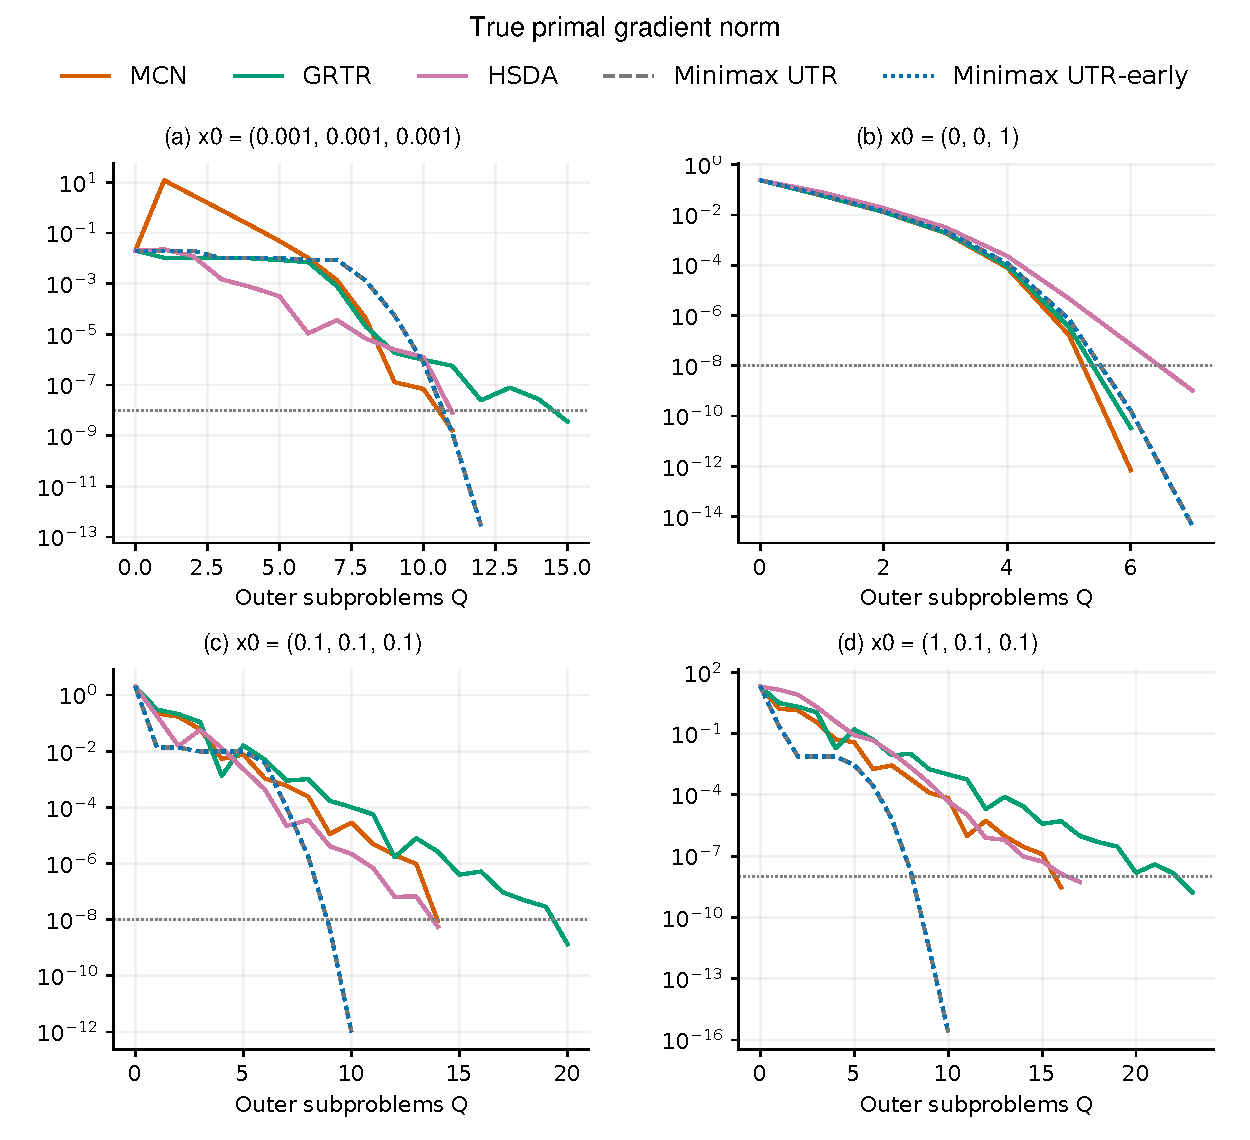
\includegraphics[width=0.90\linewidth]{figures/experiments/A_stationarity.pdf}
\caption{A: true gradient norm versus $Q$ at all four starts.
Baselines end at first hit; UTR retains native termination. Full/early
UTR overlap. Actual nonmonotonicity is retained; no running minimum.}
\label{fig:wshape-benchmark}
\end{figure}

\subsection{Benchmark B: amortized inner work}
\label{sec:exp-b}

For $x=(u,v)$, define the curved-valley payoff
\begin{align}
 P_0(u,v)&=\sqrt{1+(u-35)^2}-1+0.35[1-\cos(0.7(u-35))]
                 +\log\cosh(v-h(u)),\nonumber\\
 h(u)&=0.8\sin(u/2)+0.4\sin(\sqrt2u/2),\qquad
 C=2^{-1/2}\begin{pmatrix}1&1\\1&-1\end{pmatrix},\nonumber\\
 f_D(x,y)&=P_0(x)+0.1\sum_{i=1}^2[1-\cos((Cx)_i+d_i y_i)]
                    -3\|Dy\|^2,
 \label{eq:exp-b-payoff}
\end{align}
where $D=\operatorname{diag}(d_1,d_2)$ is invertible. The base instance
uses $D=I$, $x_0=y_0=0$, $\epsilon=10^{-6}$, and bounds
$(\ell,\mu,L_y,\rho,\bar M_P)=(6.2,5.9,6.1,4.32283,4.14516)$.
The nonlinear inner maximizer satisfies
$0.1\sin((Cx)_i+z_i^*)=6z_i^*$ for $z=Dy$; hence $|z_i^*|\le1/60$.
Online derivatives require no root solve. Roots are used only for
exact-primal controls and offline evaluation; $P\ne P_0$ and $P^*$ is
not assumed known.

Oracle-error scaling, exact-path reproduction, and exact-MCN
outer-scale controls are retained as auxiliary checks in
\Cref{app:exp-b-controls}; they do not isolate the source of tracking savings.

\paragraph{B1: reusing curvature calibration.}
Freeze exact UTR's 47 accepted points and incoming scales $\sigma_t$.
For $D_\gamma=\operatorname{diag}(\gamma^{-1/2},\gamma^{1/2})$,
$\gamma\in\{1,2,4,8\}$, the primal is unchanged. Recount all work from
zero and require the same intrinsic target at every point:
\begin{equation}
 \|D_\gamma^{-1}\nabla_yf_{D_\gamma}(x_t,y_t)\|\le r_t,
 \qquad r_t=\frac{c_0\ell\sqrt\epsilon}{4\sigma_t}.
 \label{eq:exp-b-intrinsic}
\end{equation}
The external scheduler knows $\ell$; SCAR does not. Solvers update in
$y$, without preconditioning, and AGD receives
$L_{y,\gamma}=6.1\gamma$, $\mu_\gamma=5.9/\gamma$.
Persistent SCAR-early retains $y,\nu,\mathcal M$; warm restart retains
only $y$; cold restart resets both. All checks and secants are charged.

\begin{table}[tb]
\centering\small
\setlength{\tabcolsep}{4.5pt}
\begin{tabular}{rrrrrrr}
\toprule
$\gamma$ & $\bar\kappa_y$ & Persistent & Warm restart & Cold restart & Warm AGD & Cold AGD\\
\midrule
1 & 1.03 & 462 & 391 & 445 & 195 & 187\\
2 & 4.14 & 632 & 679 & 787 & 1,068 & 1,255\\
4 & 16.54 & 1,439 & 5,837 & 6,316 & 2,566 & 3,017\\
8 & 66.17 & 3,654 & 17,297 & 18,325 & 5,492 & 6,439\\
\bottomrule
\end{tabular}
\caption{B1: fixed-path $N_y^{\rm path}$ at identical intrinsic targets.
The three restart columns use SCAR-early; AGD knows the analytic
conditioning bounds. The primal and outer path are unchanged.}
\label{tab:exp-b-conditioning}
\end{table}

At $\gamma=1$, persistent full SCAR costs 17,021 queries versus 462
for early, a factor of 36.84. AGD is still cheaper, and persistence
itself costs more than warm restart. At $\gamma=8$, persistence instead
saves a factor of 4.73 over warm restart. Downward curvature corrections
$\nu\leftarrow\nu/4$ number 2/89/92 for persistent/warm/cold restart
(1/44/46 at $\gamma=4$). Only 46 of the 13,643 saved queries at
$\gamma=8$ are secant savings; the rest includes all halving and checking
work, not solely curvature identification. All 940 returned points
satisfy the common target. This supports reuse of curvature calibration, not removal of an
accuracy logarithm or uniform superiority to AGD. Replay excludes rejected trials and outer validation, so 462
and the full-run cost 779 are distinct quantities.

\paragraph{B2: restoring accuracy under joint refinement.}
To separate warm starts from resetting curvature, fix $D=\mathrm{diag}(1/2,2)$
and subdivide each of the same 46 path segments into
$m\in\{1,2,4,8,16,32\}$ equal pieces. There are $T_m=46m+1$
requests, with $\epsilon_m=10^{-3}/m^2$ and the common native target
\[
 \|f_y\|\le\tau_m=\frac{c_0(24.5)\sqrt{\epsilon_m}}{4\bar\sigma}
       =\frac{1.7514703\times10^{-4}}{m},\qquad
 \bar\sigma=0.26998732,\quad c_0=2^{-12}.
\]
Warm-PSCAR carries $y$ forward; Cold-PSCAR starts each request at zero.
\emph{Both retain their own curvature states and use ordinary SCAR,
with early return disabled}. Warm/cold AGD use the same fixed
$(L_y,\mu_y)=(24.4,1.475)$ and reset momentum each request.
Each method and mesh starts with a fresh state. These are artificial
moving-target requests, not native UTR iterations.

Since $\|f_y(x',y)-f_y(x,y)\|\le.2\|x'-x\|$, warm starts satisfy
$R_{\rm in}/\tau_m\le1+.2\|X_{j+1}-X_j\|/\tau_{\rm ref}$,
independent of $m$. At a fixed nonzero cold residual the ratio instead
grows as $m$. We report this entry burden alongside actual queries
(\Cref{fig:exp-b-restoration}), rather than interpreting the sufficient
budget $\lceil\log_2(R_{\rm in}/\tau_m)\rceil_+$ as an observed count
or a lower bound.
From $m=1$ to 16, queries per request change from $859$ to $883$
for Warm-PSCAR and $1{,}012$ to $1{,}485$ for Cold-PSCAR;
AGD changes from $39.3$ to $40.7$ and $48.8$ to $69.9$, respectively.
Neither PSCAR arm makes a downward-$\nu$ correction.
This separates accuracy restoration from repeated initialization of curvature;
ordinary SCAR remains much more expensive than known-bound AGD.
At $m=32$, Warm-PSCAR uses $890$ queries per request; Cold-PSCAR
completes only $1299/1473$ requests within the frozen $2\times10^6$-query
budget and is excluded from full-path averages.

\begin{figure}[tb]
\centering
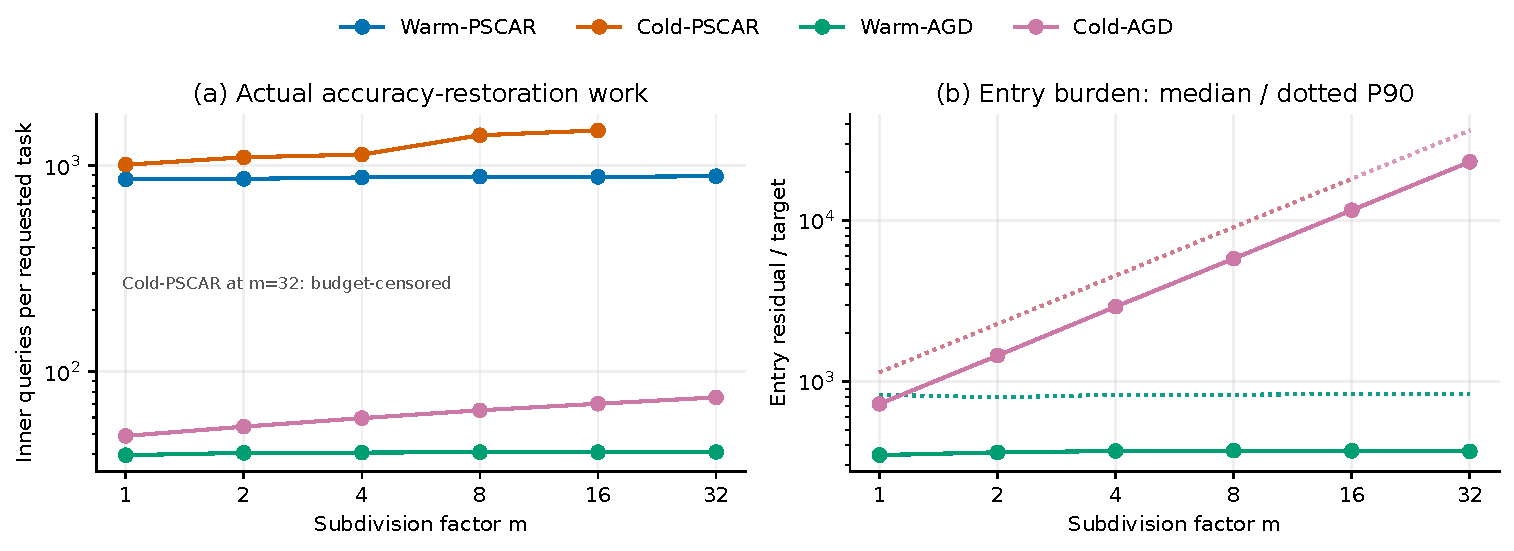
\includegraphics[width=\linewidth]{figures/experiments/B_accuracy_restoration.pdf}
\caption{B2: actual average work and relative entry residual under joint
path/accuracy refinement. Solid curves in the right panel are medians;
dotted curves are 90th percentiles. Both PSCAR arms retain curvature
state. Only complete paths enter the average-cost curves; cold entry residuals
coincide by construction.}
\label{fig:exp-b-restoration}
\end{figure}

\paragraph{B3: work along the native algorithm.}
Finally, run \Cref{alg:gradient-scaled-scar} on the same $D$, from zero,
for $\epsilon=10^{-3},\ldots,10^{-7}$, using ordinary SCAR,
$c_0=2^{-12}$, the prescribed fixed halving counts, and native validation.
A float64 trial reached its residual floor before completing its scheduled
halvings; we retain that failure and use 100-digit arithmetic for this
five-run audit, without replacing the schedule by early or target stopping.
All five 100-digit runs terminate and pass independent gradient checks,
using $215{,}781$, $189{,}531$, $173{,}125$, $308{,}127$, and $292{,}759$
queries, respectively. Accepted-trial tracking accounts for $94.9$--$97.5\%$.
These full-SCAR costs are distinct from early-return costs; changing
$\sigma_0$ with $\epsilon$ also changes the realized outer path.
We partition every query into initialization, accepted/rejected trials,
refresh, failed validation, terminal trial, or successful validation.
For ordinary accepted steps, the recorded counts satisfy
$S_{\rm tr}\le16K+\epsilon^{-3/2}C_3$, where
$C_3=\sum\sigma_k^3\|d_k\|^3$; normal returns also satisfy $Q=K+J+1$.
These are implementation/accounting checks, not evidence that the bound
is tight or that five precision settings establish a complexity rate.

\subsection{Benchmark C: robust RBF classification}
\label{sec:exp-c}

We use WDBC's 569 samples and 30 features, with a seed-2026 stratified
split into 455 training and 114 test samples. Standardization is fitted
only on training data; test labels are not used for selection.
With five trainable centers $u_j\in\mathbb R^{30}$, let
\[
 s_x(a)=\sum_{j=1}^5\tanh(v_j)e^{-\|a-u_j\|^2/8}+\tanh(v_0),
 \qquad x\in\mathbb R^{156}.
\]
For labels $b_i\in\{-1,1\}$ and unconstrained sample-wise perturbations
$z_i=\sqrt n\,y_i$, $n=455$, we minimize the maximum over
$y\in\mathbb R^{455\times30}$ of
\begin{equation}
 f(x,y)=\frac1n\sum_{i=1}^n
 \left[\log(1+e^{-b_i s_x(a_i+\sqrt n\,y_i)})
                  -\|\sqrt n\,y_i\|^2\right]
                  +\frac{10^{-4}}2\|x\|^2.
 \label{eq:exp-c-payoff}
\end{equation}
The bandwidth and adversarial penalty are fixed at 2. Separability
requires only $30\times30$ inner blocks and a $156\times156$ Schur
Hessian. All methods use $y_0=0$ and the same frozen negative-curvature
start, selected geometrically from 33 predetermined candidates, without
algorithm outcomes: initially $P=.8783993$, $\|\nabla P\|=.1371588$,
and $\lambda_{\min}=-.1574913$ (\Cref{app:exp-c-initialization}).

\paragraph{Practical calibration.}
Both baselines use warm-start AGD with restarted momentum,
$L_y=3.25$, $\mu_y=.175188$, step $1/L_y$, and momentum
$(\sqrt{L_y/\mu_y}-1)/(\sqrt{L_y/\mu_y}+1)$. We search
\begin{equation}
\begin{aligned}
 M&\in\{10^{-4},10^{-3},10^{-2},10^{-1},1,10\} &&\text{(MCN)},\\
 \widetilde L_2&\in\{10^{-4},10^{-3},10^{-2},10^{-1},1\} &&\text{(GRTR)},\\
 \tau_{\rm inner}&\in\{10^{-10},10^{-8},10^{-6},10^{-4},10^{-2}\}
                                                       &&\text{(both)}.
\end{aligned}
\label{eq:exp-c-grid}
\end{equation}
Inner stopping requires $\|\nabla_y f\|\le\tau_{\rm inner}$ in the
normalized coordinates. MCN uses cubic coefficient $M/6$. GRTR sets
$\sigma_{\rm reg}=\sqrt{\widetilde L_2}/2$ and
$r=1/(4\sqrt{\widetilde L_2})$. Its radius is
$r\sqrt{\max\{\|g_{\rm raw}\|,\epsilon\}}$; the Hessian shift is
$\sigma_{\rm reg}\sqrt{\|g_{\rm raw}\|}I$.
These practical tolerances do not carry the original oracle-error
certificates. Each of 55 configurations has budgets $Q\le10^4$,
$N_y\le10^6$, and 900 online seconds. Selection minimizes
$(N_y^{\rm hit},Q^{\rm hit})$ with fixed tie order, using only the true
gradient target $10^{-6}$. Native flags do not certify external success;
independent evaluation and stagnation handling are specified in
\Cref{app:exp-c-stopping}.

\begin{table}[tb]
\centering\small
\setlength{\tabcolsep}{5pt}
\begin{tabular}{llrrr}
\toprule
Method & Configuration & $Q^{\rm hit}$ & $N_y^{\rm hit}$ & $\|\nabla P\|_{\rm hit}$\\
\midrule
Minimax UTR-early & Fixed & 154 & 1,186 & $3.19\cdot10^{-7}$\\
MCN & $M=10^{-3},\ \tau=10^{-4}$ & 93 & 563 & $9.06\cdot10^{-8}$\\
GRTR & $\widetilde L_2=10^{-4},\ \tau=10^{-4}$ & 30 & 356 & $9.26\cdot10^{-7}$\\
\bottomrule
\end{tabular}
\caption{C: initialization-inclusive first-hit costs. Baselines are
selected on this same instance. All hit values satisfy
$P\approx.493433306$, $\lambda_{\min}\approx6.48\cdot10^{-4}$;
this does not certify global optimality. Search costs are separate.}
\label{tab:exp-c-hits}
\end{table}

The selected MCN/GRTR use 52.5\%/70.0\% fewer queries than fixed
Minimax UTR-early (\Cref{tab:exp-c-hits}), and neither selected baseline
rebounds above $10^{-6}$ after first hit. MCN nevertheless first raises
$P$ to 5.6712 (\Cref{fig:exp-c-trajectories}). Of the practical grids,
20/30 MCN and 18/25 GRTR settings hit; all $\tau=10^{-2}$ settings miss.
For GRTR at $\widetilde L_2=.01$, tightening $\tau$ from $10^{-4}$ to
$10^{-10}$ leaves $Q^{\rm hit}=229$ but raises queries from 1,073 to
10,523. More inner accuracy need not improve outer progress.

\begin{figure}[tb]
\centering
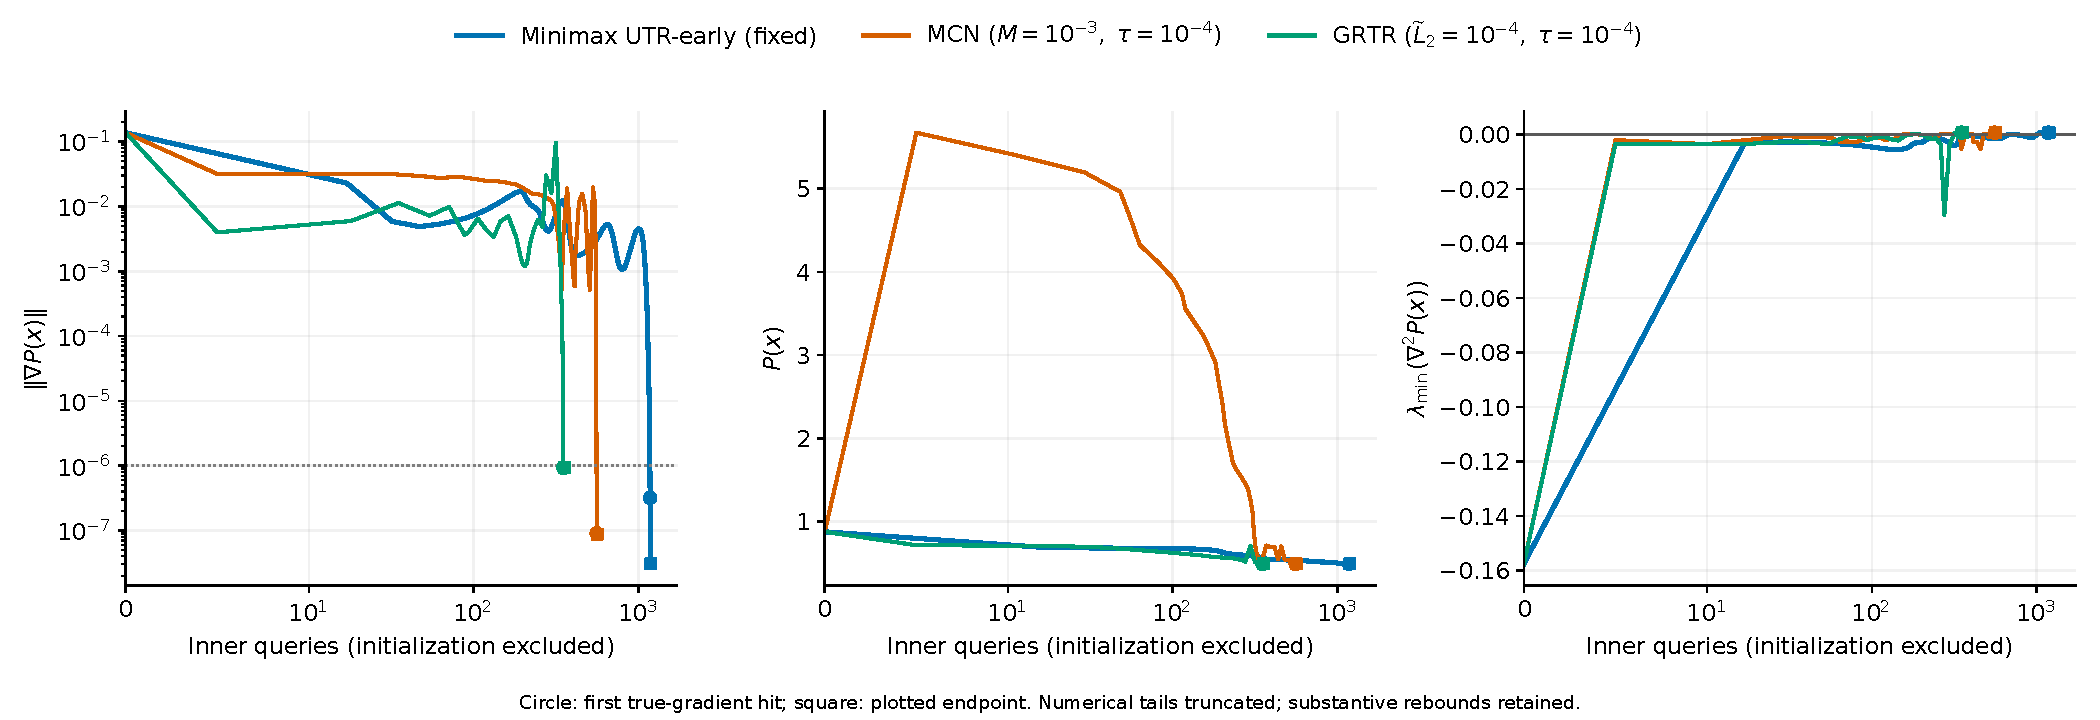
\includegraphics[width=\linewidth]{figures/experiments/C_best_three.pdf}
\caption{C: true gradient, objective, and minimum Hessian eigenvalue.
Plots subtract initialization (10 queries for UTR, 6 per baseline);
tables include it. Circles denote first hit, squares display endpoints.
The symmetric-log axis retains zero. Only terminal numerical tails are
trimmed; actual rebounds remain (\Cref{app:exp-c-stopping}).}
\label{fig:exp-c-trajectories}
\end{figure}

Formula-scale MCN/GRTR references with $M\approx1.0373\cdot10^7$ and
$L_2\approx2.0281\cdot10^6$ still have gradient norms .01485/.17086
after 10,000 subproblems. They also use different inner dynamics and
formula-derived tolerances; this contrast is not solely an outer-scale
effect. The supplied joint $\rho=73.10$ was not independently globally
certified (\Cref{app:exp-c-reference}).

Together, A demonstrates outer progress, B identifies inner-work
mechanisms and their limits, and C shows the competitiveness of
instance-tuned fixed-scale methods. We do not infer uniform empirical
dominance, transfer of selected parameters to unseen starts, or improved
test accuracy from these optimization experiments.


\section{Conclusion}
\label{sec:conclusion}

The parameter-free minimax method is a direct oracle realization
of an inexact UTR theorem for general unconstrained optimization.
The theorem separates the construction of approximate values and
derivatives from outer progress; its supporting estimates provide
the path and stored-value bounds needed for inner-work analysis.
Corrected envelope oracles and persistent SCAR satisfy its
hypotheses in the NC--SC setting, yielding leading complexities
$O(\Delta_P\kappa^{3/2}\sqrt\rho\,\epsilon^{-3/2})$ and
$O(\Delta_P\kappa^2\sqrt\rho\,\epsilon^{-3/2})$ for outer
subproblems and inner-gradient evaluations, respectively.

The guarantee holds uniformly over each class with fixed common
regularity constants once $\epsilon$ is sufficiently small.
The algorithm does not certify that it has entered this regime.
An observable all-accuracy certificate and a treatment of inexact
trust-region solves remain beyond the present analysis.


\clearpage
\appendix
\section{Proof of the inexact UTR theorem}
\label{app:adaptive-utr-proofs}

All results in this appendix concern the general unconstrained
objective $F$ and the oracle interface of
\Cref{ass:inexact-oracle}.  No minimax structure is used.

We first record the auxiliary estimates used by the minimax analysis.
For this appendix, write $F^*=\inf_xF(x)$,
$\Delta_F=F(x_0)-F^*$, $h_0=\max\{\|\widehat g_0\|,\epsilon\}$,
and $\bar\sigma=\max\{\sigma_0,2\sqrt{M/6}\}$, where
$\widehat g_0$ is the initialized working gradient.  Define
\begin{equation}\label{eq:utr-budget}
\begin{aligned}
 B_\epsilon:={}&\Delta_F+
 \frac{23C_v\epsilon^{3/2}}{7\sigma_0^3}\\
 &+\frac{\epsilon^{3/2}}{512\sigma_0}
 \left[\left\lceil\log_2\frac{h_0}{\epsilon}\right\rceil
       +1+\log_2\left(1+\frac{5C_g}{4\sigma_0^2}\right)\right].
\end{aligned}
\end{equation}

\begin{proposition}[Counting and path estimates]\label{prop:utr-budgets}
Under the hypotheses of \Cref{thm:total-complexity}, every generated
scale is at most $\bar\sigma$.  If $K,J,Q$ denote, respectively,
the numbers of accepted trials, failed trials, and solved
subproblems at termination, then
\begin{equation}\label{eq:utr-counts}
 K\le1024\bar\sigma B_\epsilon\epsilon^{-3/2},\qquad
 J\le\left\lceil\log_2\max\left\{1,
          \frac{\sqrt{M/6}}{\sigma_0}\right\}\right\rceil,
 \qquad Q=K+J+1.
\end{equation}
There are at most $J+1$ validation calls.  Every stored iterate and
every finite prefix of accepted steps satisfy
\begin{equation}\label{eq:utr-path-budget}
 F(x)-F^*\le B_\epsilon,\qquad
 \sum_{\rm accepted}\sigma_k^2\|d_k\|^3\le8B_\epsilon.
\end{equation}
The bounds on $K$ and $J$ also hold for every finite prefix.
\end{proposition}

We prove the proposition together with \Cref{thm:total-complexity}
at the end of this appendix.

\subsection{A common trust-region estimate}
\label{app:common-tr-estimate}

\begin{lemma}[Common inexact trust-region step estimate]
\label{lem:common-inexact-tr-step}
Let $F:\R^n\to\R$ be twice continuously differentiable with an
$M$-Lipschitz Hessian, $M>0$.  At a point $x$, let $g$ and a
symmetric $H$ satisfy
\[
 \|g-\nabla F(x)\|\le\delta_0,
 \qquad
 \|H-\nabla^2F(x)\|\le\xi.
\]
For $a\ge0$ and $R>0$, let $d$ be a global solution of
\[
 \min_{\|u\|\le R}\;
 q(u):=g^Tu+\frac12u^T(H+aI)u,
\]
let $\lambda$ be the multiplier supplied by
\eqref{eq:tr-global-optimality}, and write $r=\|d\|$.  Let a candidate
gradient $g^+$ satisfy
$\|g^+-\nabla F(x+d)\|\le\delta_+$.  Then
\begin{subequations}\label{eq:common-tr-estimates}
\begin{align}
 F(x)-F(x+d)
 &\ge\frac{a-\xi}{2}r^2+\frac{\lambda}{2}r^2
      -\frac M6r^3-\delta_0r,
       \label{eq:common-function-bound}\\
 \|g^+\|
 &\le(a+\xi+\lambda)r+\frac M2r^2+\delta_0+\delta_+.
       \label{eq:common-gradient-bound}
\end{align}
\end{subequations}
\end{lemma}

\begin{proof}
Apply \eqref{eq:tr-global-optimality} with $B=H+aI$.  Its stationarity
and positive-semidefiniteness conditions give
\[
 q(d)=-\frac12d^T(H+aI)d-\lambda r^2
 \le-\frac{\lambda}{2}r^2,
\]
and Hessian Lipschitz continuity gives the standard Taylor estimates
\citep[Lemma~1.2.4]{nesterov2004introductory}
\[
\begin{aligned}
 \|\nabla F(x+d)-\nabla F(x)-\nabla^2F(x)d\|
 &\le\frac M2r^2,\\
 F(x+d)-F(x)-\nabla F(x)^Td-\frac12d^T\nabla^2F(x)d
 &\le\frac M6r^3.
\end{aligned}
\]
The second estimate and the current endpoint errors imply
\[
 F(x)-F(x+d)
 \ge-g^Td-\frac12d^THd-\delta_0r-\frac{\xi}{2}r^2-\frac M6r^3.
\]
Since
$-g^Td-d^THd/2=-q(d)+ar^2/2$, the model bound yields
\eqref{eq:common-function-bound}.

For the candidate gradient, decompose the two endpoint errors, Taylor
remainder, Hessian error, and model residual:
\begin{align*}
g^+
&=[g^+-\nabla F(x+d)]
 +[\nabla F(x+d)-\nabla F(x)-\nabla^2F(x)d]\\
&\quad+[\nabla F(x)-g]
 +[\nabla^2F(x)-H]d+[g+Hd].
\end{align*}
The stationarity part of \eqref{eq:tr-global-optimality}, again with
$B=H+aI$, gives $g+Hd=-(a+\lambda)d$.  Taking norms proves
\eqref{eq:common-gradient-bound}.
\end{proof}


\subsection{Safe-scale acceptance and validation}

\begin{lemma}[Safe scale for inexact UTR]
\label{lem:utr-safe}
Under the hypotheses of \Cref{thm:total-complexity}, the following hold
for every generated trial of \Cref{alg:adaptive-utr}.
If $\sigma^2\ge M/6$, every ordinary trial of
\Cref{alg:adaptive-utr} satisfies both acceptance tests, and
every trial with $h=\epsilon$ and $r<R(h,\sigma)$ passes validation.
At any scale $\sigma\ge\sigma_0$, successful validation implies
\begin{equation}\label{eq:utr-validator-return}
 \|\nabla F(x^+)\|<\epsilon,
 \qquad
 \lambda_{\min}(\nabla^2F(x^+))
 \ge-\frac{85}{32}\sigma\sqrt\epsilon.
\end{equation}
\end{lemma}

\begin{proof}[Proof of \Cref{lem:utr-safe}]
Apply \Cref{lem:common-inexact-tr-step} to $F$ with
\[
 a=\sigma\sqrt h+\frac{\sigma\sqrt\epsilon}{64},
 \qquad
 \xi=\frac{\sigma\sqrt\epsilon}{64},
 \qquad
 \delta_0=\delta_+=\frac{\epsilon}{1024}.
\]
The endpoint errors follow from \eqref{eq:utr-safe-errors}.
Since $r\le\sqrt h/(4\sigma)$ and $M\le6\sigma^2$,
\[
 \frac{M}{6}r^3\le\frac W4.
\]
Thus \eqref{eq:common-function-bound} gives
\[
 F(x)-F(x+d)\ge\frac W4+\frac U2-\frac{\epsilon r}{1024}.
\]
Young's inequality and $h\ge\epsilon$ imply
\[
 \frac{\epsilon r}{1024}
 \le\frac W8+
       \frac{2\epsilon^2}{1024^2\sigma\sqrt h}
 \le\frac W8+\frac{2T}{1024^2}.
\]
After paying the two working-value errors,
\[
 \widehat F-\widehat F^+
 \ge\frac W8+\frac U2
       -\left(\frac{2}{1024^2}+\frac{2}{4096}\right)T
 \ge\frac W8+\frac U4-\frac T{1024}.
\]
For the gradient test, \eqref{eq:common-gradient-bound} gives
\[
 \|\widehat g^+\|
 \le\lambda r+\frac h4+\frac h{128}
                    +\frac{3h}{16}+\frac h{512}
 =\lambda r+\frac{229h}{512}
 \le\lambda r+\frac h2.
\]
Hence every ordinary trial is accepted at a safe scale.

If $h=\epsilon$ and $r<R(h,\sigma)$, complementarity gives
$\lambda=0$, and the model shift is
$a=(65/64)\sigma\sqrt\epsilon$.  Applying
\eqref{eq:common-gradient-bound} to the true endpoint gradient
($\delta_+=0$), with
$\delta_0=\epsilon/1024$ and $\xi=\sigma\sqrt\epsilon/64$,
gives
\[
 \|\nabla F(x+d)\|
 \le\left(\frac{66}{256}+\frac3{16}+\frac1{1024}\right)\epsilon
 =\frac{457}{1024}\epsilon.
\]
Moreover, model positive semidefiniteness, the current Hessian error,
and Hessian Lipschitz continuity imply
\begin{align*}
 \lambda_{\min}(\nabla^2F(x+d))
 &\ge-a-\xi-Mr\\
 &\ge-\left(\frac{66}{64}+\frac32\right)\sigma\sqrt\epsilon
 =-\frac{81}{32}\sigma\sqrt\epsilon.
\end{align*}
The validation error bounds therefore give
\[
 \|g_{\rm v}\|\le\frac{458}{1024}\epsilon,
 \qquad
 \lambda_{\min}(H_{\rm v})
 \ge-\frac{82}{32}\sigma\sqrt\epsilon,
\]
so validation succeeds.  At any generated scale, a successful
validation and \eqref{eq:utr-validation-errors} imply
\[
 \|\nabla F(x^+)\|
 \le\frac\epsilon2+\frac\epsilon{1024}<\epsilon,
 \qquad
 \lambda_{\min}(\nabla^2F(x^+))
 \ge-\left(\frac{21}{8}+\frac1{32}\right)\sigma\sqrt\epsilon.
\]
This proves \eqref{eq:utr-validator-return}.
\end{proof}


\subsection{Accepted-step and scale-refresh budgets}

For $h\ge\epsilon$, define the gradient level and stored potential
\begin{equation}\label{eq:utr-potential}
 \mathcal L_\epsilon(h):=\left\lceil\log_2(h/\epsilon)\right\rceil,
 \qquad
 \Phi:=\widehat F+\frac{\epsilon^{3/2}}{512\sigma}
                           \mathcal L_\epsilon(h).
\end{equation}


\begin{lemma}[Accepted-step potential decrease]
\label{lem:utr-descent}
Every ordinary accepted step of
\Cref{alg:adaptive-utr} satisfies
\begin{equation}\label{eq:utr-potential-decrease}
 \Phi-\Phi^+\ge\frac W{32}+\frac T{1024}+\frac U{16},
\end{equation}
where the scale is unchanged and $\Phi$ is defined by
\eqref{eq:utr-potential}.
\end{lemma}

\begin{proof}
First note that if $h>\epsilon$ and
$h^+\le\max\{h/2,\epsilon\}$, then
\begin{equation}\label{eq:utr-layer-halving}
 \mathcal L_\epsilon(h^+)\le\mathcal L_\epsilon(h)-1.
\end{equation}
For $\epsilon<h\le2\epsilon$, the two levels are $1$ and $0$.
For $h>2\epsilon$, the result follows from
$\lceil t-1\rceil=\lceil t\rceil-1$.
We will also use, for $c\ge1$ and $h^+\le ch$,
\begin{equation}\label{eq:utr-layer-growth}
 \mathcal L_\epsilon(h^+)-\mathcal L_\epsilon(h)
 \le\lceil\log_2c\rceil\le1+\log_2c.
\end{equation}

Suppose first that the accepted step is interior.  Then $\lambda=0$
and $U=0$.  Since this is an ordinary trial, $h>\epsilon$.
The gradient acceptance test implies
$h^+\le\max\{h/2,\epsilon\}$, so \eqref{eq:utr-layer-halving} and
the value test yield
\[
 \Phi-\Phi^+\ge\frac W8-\frac T{1024}+\frac T{512}
 =\frac W8+\frac T{1024}.
\]
This proves \eqref{eq:utr-potential-decrease} in the interior case.

For a boundary step, put $z=\lambda r/h$.  The gradient test gives
$h^+/h\le\max\{1,1/2+z\}$.  By \eqref{eq:utr-layer-growth},
\[
 \mathcal L_\epsilon(h^+)-\mathcal L_\epsilon(h)
 \le1+\log_2\max\{1,1/2+z\}
 \le1+\frac z{\ln2}.
\]
Since $r=\sqrt h/(4\sigma)$,
\[
 W=\frac{h^{3/2}}{16\sigma}\ge\frac T{16},
 \qquad
 U=\frac{zh^{3/2}}{4\sigma},
 \qquad Tz\le4U.
\]
Consequently,
\begin{align*}
 \Phi-\Phi^+
 &\ge\frac W8+\frac U4-\frac T{1024}
       -\frac T{512}\left(1+\frac z{\ln2}\right)\\
 &\ge\frac W8+
       \left(\frac14-\frac1{128\ln2}\right)U
       -\frac{3T}{1024}\\
 &\ge\frac{5W}{64}
       +\left(\frac14-\frac1{128\ln2}\right)U.
\end{align*}
Finally,
$5W/64\ge W/32+T/1024$ and
$1/4-1/(128\ln2)\ge1/16$, proving the claim.
\end{proof}

To account for changes of scale, define
\begin{equation}\label{eq:utr-budget-parameters}
\begin{aligned}
 E(\sigma)&:=C_v\frac{\epsilon^{3/2}}{\sigma^3},
 &E_0&:=E(\sigma_0),
 &T_0&:=\frac{\epsilon^{3/2}}{\sigma_0},\\
 \mathcal L_0&:=\mathcal L_\epsilon(h_0),
 &D_0&:=1+\log_2\left(1+\frac{5C_g}{4\sigma_0^2}\right).
\end{aligned}
\end{equation}
The budget in \eqref{eq:utr-budget} can therefore be written as
\[
 B_\epsilon=\Delta_F+\frac{23}{7}E_0+
                \frac{T_0}{512}(\mathcal L_0+D_0).
\]
Write $\sigma_*:=\sqrt{M/6}$.  Every failed trial doubles $\sigma$,
and \Cref{lem:utr-safe} excludes failures at or above $\sigma_*$.
If $\sigma_0\ge\sigma_*$ there are no failures.  Otherwise, at most
$\lceil\log_2(\sigma_*/\sigma_0)\rceil$ doublings are possible.
Consequently every finite prefix satisfies
\begin{equation}\label{eq:utr-inexact-scale-bound}
 J\le\left\lceil\log_2\max\{1,\sigma_*/\sigma_0\}\right\rceil,
 \qquad
 \sigma\le\bar\sigma:=\max\{\sigma_0,2\sigma_*\}.
\end{equation}

\begin{lemma}[Cumulative accepted-step budget]
\label{lem:utr-cumulative-budget}
Under the preceding conditions, every finite prefix satisfies
\begin{equation}\label{eq:utr-cumulative-budget}
 \sum_{\rm accepted}
 \left(\frac{W_k}{32}+\frac{T_k}{1024}+\frac{U_k}{16}\right)
 \le B_\epsilon.
\end{equation}
Every stored iterate satisfies $F(x)-F^*\le B_\epsilon$.
\end{lemma}

\begin{proof}
At a refresh, $x$ is unchanged and the scale goes from $\sigma$ to
$2\sigma$.  By \eqref{eq:utr-working-errors}, the working-value jump
is at most
\[
 E(\sigma)+E(2\sigma)=\frac98E(\sigma).
\]
The scales at failures form a doubling sequence, so the sum of all
positive value jumps is at most
\[
 \frac98E_0\sum_{j\ge0}2^{-3j}=\frac97E_0.
\]
For the gradient-level term, the two working-gradient errors give
\[
 \|\widehat g_{\rm new}-\widehat g_{\rm old}\|
 \le\frac{5C_g\epsilon}{4\sigma^2}.
\]
The map $g\mapsto\max\{\|g\|,\epsilon\}$ is $1$-Lipschitz and
$h_{\rm old}\ge\epsilon$.  Hence
\[
 \frac{h_{\rm new}}{h_{\rm old}}
 \le1+\frac{5C_g}{4\sigma^2},
 \qquad
 \mathcal L_\epsilon(h_{\rm new})
       -\mathcal L_\epsilon(h_{\rm old})\le D_0.
\]
Write $\mathcal L_{\rm old}$ and $\mathcal L_{\rm new}$ for these
two levels.  Since $T_{\rm new}=T_{\rm old}/2$ and the levels are
nonnegative, the positive jump of the level contribution is at most
\[
 \left[
  \frac{T_{\rm old}}{1024}
  (\mathcal L_{\rm new}-2\mathcal L_{\rm old})
 \right]_+
 \le\frac{T_{\rm old}D_0}{1024}.
\]
Its cumulative positive jump is therefore bounded by
\[
 \frac{T_0D_0}{1024}\sum_{j\ge0}2^{-j}
 =\frac{T_0D_0}{512}.
\]

The initial potential is at most
$F(x_0)+E_0+T_0\mathcal L_0/512$, and every stored potential is at
least $F^*-E_0$.  Telescoping \eqref{eq:utr-potential-decrease} and
paying the two refresh bounds gives
\[
 \sum_{\rm accepted}
 \left(\frac W{32}+\frac T{1024}+\frac U{16}\right)
 \le\Delta_F+2E_0+\frac97E_0
       +\frac{T_0}{512}(\mathcal L_0+D_0)=B_\epsilon.
\]
The same upper bound on the stored potential, together with
$F(x)\le\Phi+E_0$, gives $F(x)-F^*\le B_\epsilon$.

\end{proof}

\subsection{Termination and the theorem's conclusions}

\begin{proof}[Proof of \Cref{thm:total-complexity,prop:utr-budgets}]
Every oracle call is finite by the interface assumptions.  By
\Cref{lem:utr-safe}, failed trials can occur only below
$\sqrt{M/6}$, and the scale bound
\eqref{eq:utr-inexact-scale-bound} limits their number uniformly
over all finite prefixes.  Since
$T_k\ge\epsilon^{3/2}/\bar\sigma$, \Cref{lem:utr-cumulative-budget}
gives, for every finite prefix,
\[
 K\frac{\epsilon^{3/2}}{1024\bar\sigma}\le B_\epsilon.
\]
Every nonterminal trial is either accepted or failed.  Hence an
infinite run would contradict one of these finite-prefix bounds,
and the algorithm terminates.

At termination, there have been $K$ accepted trials, $J$ failed
trials, and one successful validation trial, each solving one
subproblem.  Thus $Q=K+J+1$, proving \eqref{eq:utr-counts}.
Every validation either terminates or causes a failed trial, so
there are at most $J+1$ validation calls.
The returned-point estimate \eqref{eq:utr-validator-return} and
$\sigma\le\bar\sigma$ prove \eqref{eq:return-guarantee}.
For the cubic-path estimate, the radius constraint gives
\[
 4\sigma_k^2r_k^3\le\sigma_k\sqrt{h_k}\,r_k^2=W_k.
\]
Thus \Cref{lem:utr-cumulative-budget} implies
$\sum_{\rm accepted}\sigma_k^2r_k^3\le8B_\epsilon$ for every
finite prefix.  Its stored-value estimate supplies the other part
of \eqref{eq:utr-path-budget}, proving \Cref{prop:utr-budgets}.

To obtain the total count \eqref{eq:utr-total-count}, the initial
working-gradient bound gives
\[
 \frac{h_0}{\epsilon}
 \le\max\left\{1,
       \frac{\|\nabla F(x_0)\|}{\epsilon}
          +\frac{C_g}{\sigma_0^2}\right\}.
\]
Consequently the bracket in \eqref{eq:utr-budget} is at most a
universal constant times
$\log(e+\|\nabla F(x_0)\|/\epsilon+C_g/\sigma_0^2)$.
Substitute this estimate and
$\bar\sigma\le\max\{\sigma_0,\sqrt M\}$ into
\eqref{eq:utr-counts}.  The terminal $+1$ is absorbed because this
logarithm and $\max\{\sigma_0,\sqrt M\}/\sigma_0$ are both at least
one, and the bound on $J$ is
$O(1+\log(1+\sqrt M/\sigma_0))$.
This gives \eqref{eq:utr-total-count} and completes the theorem.
\end{proof}


\section{Persistent SCAR}
\label{app:scar-tool-proof}

\begin{proof}[Derivation of \Cref{thm:scar-blackbox}]
For $u^*=\arg\min\phi$, the cited AR theorem with initial
regularization $\nu/10$ gives
\[
 \|\nabla\phi(v)\|\le\frac\nu2\|u-u^*\|
 \le\frac\nu{2\mu}\|\nabla\phi(u)\|,
\]
where the second inequality is strong convexity.  This proves the
halving implication.  The theorem's gradient cost becomes
$O(1+\sqrt{L/\nu})$.  At each AR stage the backtracking estimate is
at most $\max\{\mathcal M_{s-1}/2,2L\}$: a trial estimate at least
$L$ satisfies the tested smoothness inequality, and backtracking
doubles its estimate only after a failed test.  Starting from
$\mathcal M\le4L$, induction gives $\mathcal M_s\le2L$ and hence
the claimed bound on $\mathcal M^+$.  The argument also covers
$L=\mu$.
\end{proof}

For completeness, the secant bounds \eqref{eq:secant-bounds-pf} follow
from strong monotonicity and Cauchy--Schwarz:
\[
 \mu\|z-u\|^2
 \le\langle\nabla\phi(z)-\nabla\phi(u),z-u\rangle
 \le\|\nabla\phi(z)-\nabla\phi(u)\|\,\|z-u\|.
\]
Dividing by $\|z-u\|^2$ gives the lower bound; the upper bound is
gradient Lipschitz continuity.

\begin{proof}[Proof of \Cref{lem:scar-persistent-half}]
The initial line-search estimate satisfies $\mathcal M_0\le4L$.
Every AR call returns $\mathcal M^+\le2L$ by
\Cref{thm:scar-blackbox}.  All objectives have the same upper
smoothness bound $L$, so this retained estimate remains admissible
even when the next objective changes.  Thus the AR guarantee applies
inductively to every attempted call.

By \Cref{thm:scar-blackbox}, a halving attempt on any $\phi_j$
must succeed whenever $\nu\le\mu$.
In particular, failure implies $\nu>\mu$ and the update after a
failure leaves $\nu>\mu/4$.  Since the initial guess satisfies
$\nu_0\ge\mu$, throughout the complete sequence we have
$\nu\ge\mu/4$.  After
$\lceil\log_4(\nu_0/\mu)\rceil$ failures, the guess is at most
$\mu$, and no later objective can cause a failure: the same
strong-convexity bound applies to every $\phi_j$.  Thus the complete
sequence has at most $\lceil\log_4(\nu_0/\mu)\rceil$ failures,
and every halving call terminates.

Each attempt uses $O(1+\sqrt{L/\nu})=O(\sqrt{L/\mu})$ gradient
evaluations because $\nu\ge\mu/4$ and $L/\mu\ge1$.
There are at most $N$ successful AR attempts and at most
$\lceil\log_4(\nu_0/\mu)\rceil$ failed attempts.
The at most $N$ initial residual queries, including queries for calls
with zero initial residual, fit in the same bound.  Summing proves
\eqref{eq:persistent-scar-count}.  Returning $u$ when
$\nabla\phi_j(u)=0$ already satisfies the required residual reduction
and does not change either retained estimate.
\end{proof}


\clearpage
\section{Published-setting MCN reproduction}
\label{app:wshape-published}

For reference, we retain the MCN experimental parameters
$M=10$, $K=8$, $\eta=0.1$, and $\theta=0.9$ with the original
21-update budget. We use the paper's Euclidean cubic model and the
same global spectral solver as in \Cref{sec:w-shaped}; this is not
a claim to reproduce every implementation detail of the released
coordinatewise cubic code. These runs are excluded from the tuned
main comparison. Each uses 168 inner-gradient queries. The target
in the table is exactly \eqref{eq:wshape-target}; a dash means no
hit within 21 updates, not nonconvergence beyond that budget.

\begin{center}
\begin{tabular}{lrrr}
\toprule
$x_0$ & First hit $T$ & Final $P-P^\star$ & Final $\|\nabla P\|$\\
\midrule
$(10^{-3},10^{-3},10^{-3})$ & -- & $5.74\cdot10^{-9}$ & $4.79\cdot10^{-4}$\\
$(0,0,1)$ & 9 & $0$ & $0$\\
$(0.1,0.1,0.1)$ & -- & $5.67\cdot10^{-5}$ & $4.76\cdot10^{-2}$\\
$(1,0.1,0.1)$ & -- & $6.64\cdot10^{-4}$ & $1.10\cdot10^{-1}$\\
\bottomrule
\end{tabular}
\end{center}
Reported zeros are floating-point values. Full trajectories are
retained in the experiment's published-setting reproduction record.

\clearpage
% Concise protocols; complete records are in the accompanying experiment archive.
\section{Experimental protocols and reproducibility}
\label{app:exp-details}

\paragraph{Implementation and accounting.}
\label{app:exp-accounting}
Historical A/B1/C use $c_0=1/128$ and an all-ones unit secant;
new B2/B3 use $c_0=2^{-12}$ and the manuscript's $e_1$ secant.
Full UTR runs initialize $\sigma_0=1/\log(e/\epsilon)$.
The charged secant initializes curvature without the strong-concavity modulus. The implemented model uses
$h=\max\{\|\widehat g\|,\epsilon\}$, radius $\sqrt h/(4\sigma)$,
and Hessian shift $\sigma\sqrt h+\sigma\sqrt\epsilon/64$.
Initial refinement targets $c_0a_0\sqrt\epsilon/(4\sigma_0)$, with
observable secant $a_0$; subsequent calls follow the recorded tracking,
refresh, and validation schedule. A uses \texttt{tracking\_mode=target}.
These operational settings are disclosed rather than identified with
every subroutine setting of the analyzed algorithm. Paired ordinary/early
runs differ only in the inner return test.

$N_y$ counts performed inner-gradient evaluations, including checks,
secants, and unsuccessful work. A's fixed-count AGD uses $K_{\rm in}$
queries per call; C's residual-stopped AGD uses $1+2k$ for $k$ updates,
plus the recorded initial query and interrupted work. A C query covers
all 455 samples. C tables charge initialization and current-point model
refinement; terminal points without a new model use arrival counts.
Figures subtract initialization and place the common $x_0$ at zero.
Schur assembly, Hessians, dense subproblem solves, and offline primal
evaluation consume work outside $N_y$. C's Minimax UTR value oracle uses
an eight-point curvature integral for small-step remainders; it does not
perform a hidden inner Newton solve. Offline roots never feed online
updates. A uses analytic primal derivatives; B uses independent scalar root solves;
C uses independent Newton solves in physical coordinates with each
unaveraged sample residual at most $10^{-12}$.

\paragraph{A: parameter searches.}
\label{app:exp-a}
At each start, selection prioritizes the common stationarity hit, then
$(Q^{\rm hit},N_y^{\rm hit})$, then fixed grid order; invalid solves are
ineligible. The following sets define the complete candidate families:
\begin{align*}
\text{MCN: }\quad M&\in\{.1,.3,1,2,3,5,10,30\},&
K_{\rm in}&\in\{4,8,12,20,40\},\\
\eta_y&\in\{.05,.1,.15,.2\},&
\theta_y&\in\{0,.5,.8,9/11,.9\};\\
\text{GRTR: }\quad K_{\rm in}&\in\{5,8,10,20\},&
\eta_y&\in\{.05,.1,.2\},\\
\theta_y&\in\{0,.5,.9\},&
(\sigma_{\rm reg},r)&\in\{.03,.1,.3,1\}\times\{.3,1,3\};\\
\text{HSDA: }\quad K_{\rm in}&\in\{4,8,12,20,40\},&
\eta_y&\in\{.05,.1,.15,.2\},\\
\theta_y&\in\{0,.5,.8,.9\},&
\alpha_H&\in\{.003,.01,.03,.1,.3\},\\
\Lambda&\in\{.03,.05,.1,.2,.3\},&
\omega_H&\in\{.05,.1,.25,.4\}.
\end{align*}
MCN exhausts 800 configurations per start. GRTR first tests 36 inner
settings at $(\sigma_{\rm reg},r)=(.1,1)$, then 12 outer settings, then
one adjacent-coordinate pass, caching duplicates: 200 distinct
configuration--start pairs overall. HSDA exhausts 8,000 settings per
start. Baseline budgets are 100 updates; MCN/GRTR stop at external
hit, while HSDA records its native flag and completes the short-step
update without stopping. Its displayed curves end at offline first hit.
Inner points are warm-started with momentum reset. The searches consume,
respectively, $2{,}920{,}692$, $132{,}327$, and $53{,}760{,}000$ queries,
excluded from selected curves. Unequal, same-start searches are not
held-out comparisons. The archive lists all selected parameters and
complete trajectories.

\paragraph{B: bounds and pathwise verification.}
\label{app:exp-b}
\label{app:exp-b-constants}
For the base payoff, bounds on the curved-valley Hessian and its
Lipschitz constant are $L_0=3.03777417$ and $M_0=4.03998631$.
The cosine term contributes at most $2\eta$ and $2\sqrt2\eta$,
respectively. With $R=6$ and $\eta=.1$, this yields
\[
 \ell=\max\{L_0,R\}+2\eta=6.2,\quad \mu=R-\eta=5.9,\quad
 \rho=M_0+2\sqrt2\eta=4.32282902.
\]
The scalar envelope
$\Psi(s)=\max_z\{\eta[1-\cos(s+z)]-Rz^2/2\}$ satisfies
$|\Psi'''|\le\eta[R/(R-\eta)]^3$, giving
$\bar M_P=4.14515772$. The MCN formula scale $28.37671254$ and
$\bar M_P$ are chosen upper bounds, not measured optimal constants.

\label{app:exp-b-controls}
At $x=(.3,-.5)$, perturb the base inner maximizer along $(1,1)/\sqrt2$
at seven scales $10^{-4}$ to $10^{-1}$. Raw-gradient, corrected-gradient,
and Schur-Hessian slopes are $.9992$, $2.0055$, and $1.0060$,
with a 70-digit cross-check. Exact UTR and Minimax UTR-early require
46 accepted updates and 48 subproblems at $\epsilon=10^{-6}$;
early costs 779 queries, with identical acceptance decisions and maximum
single-coordinate path difference $1.16\times10^{-9}$. Exact MCN requires
153/60/84 updates for $M=28.3767,\bar M_P,2\bar M_P$.
These separate outer-scale and oracle-accuracy checks are not evidence
of inner-query savings; exact root computation is not free.

Replay freezes the 47 accepted-path points and incoming scales.
The target is $r_t=c_0\ell\sqrt\epsilon/(4\sigma_t)$:
$1.79406573\times10^{-4}$ initially and $4.48516433\times10^{-5}$
thereafter. Costs restart at zero and exclude path-generation rejections
and validation. Under $z=D_\gamma y$, every solver must satisfy
$\|D_\gamma^{-1}\nabla_y f\|\le r_t$: the primal and intrinsic accuracy
are unchanged. AGD uses known $L_y=6.1\gamma$ and $\mu_y=5.9/\gamma$;
SCAR retains or resets state as specified in the main comparison.
At $\gamma=1$, persistent/warm-restart/cold-restart totals
$462/391/445$ decompose into 47 residual checks each, $1/47/47$
secants, and $414/297/351$ halving queries. Downward-$\nu$ updates
across $\gamma=1,2,4,8$ are $(0,0,1,2)$, $(0,0,44,89)$, and
$(0,0,46,92)$, respectively. These are observed state corrections,
not identification of the true modulus or an additive causal
attribution at identical inner points. All 940 returned outputs pass
their common residual target. Exact-primal controls and full-SCAR replay
are not a full minimax baseline leaderboard.

\paragraph{B2/B3: new audits.}
The original 47 points and every subdivision endpoint are preserved exactly.
B2 budgets each configuration at $2\times10^6$ queries or 1,800 seconds;
an unfinished path is reported as incomplete, with no imputed zero-cost tasks.
All checks and initial secants are charged. Stored events distinguish the
sufficient halving budget, actual successful calls, downward-$\nu$ corrections,
and smoothness backtracking. Both PSCAR arms preserve their own states, which
can differ; fixed-dynamics AGD provides an additional warm-start control.
Cold-PSCAR is not a proxy for warm-started MCN.

B3 budgets each precision at 2,000 trials, $2\times10^6$ queries, or
1,800 seconds. At $\epsilon=10^{-3}$, float64 completes 15 of 17
scheduled first-trial halvings before a residual near $6.94\times10^{-18}$
stagnates; 396,070 actual queries precede the AR iteration-limit failure.
The separate 100-digit runs keep ordinary SCAR, fixed tracking counts,
one refresh halving, and a once-fixed validation secant target. Rejection
restores the old inner point but retains updated curvature state. Online
oracles have analytic derivatives and use no exact inner root. Decimal
state/residual logs and separately charged offline roots are retained.
The five native audits give $(Q,K,J)=(44,42,1),(36,34,1),(30,28,1),
(49,46,2),(43,40,2)$ in decreasing $\epsilon$ order. Scheduled tracking
counts are $734,644,585,1031,979$; total halving calls, including refresh
and validation, are $735,646,588,1035,985$. Downward-$\nu$ corrections
are zero throughout. Final true gradients are approximately
$2.24\times10^{-7},1.42\times10^{-9},1.07\times10^{-9},
1.52\times10^{-13},2.04\times10^{-12}$.
The archive reports all seven disjoint cost categories, $C_2,C_3$, and
accounting slack. These finite tolerances are not asserted to satisfy an
unknown theorem onset threshold; 100-digit and float64 timings are not
compared as a speed benchmark.

\paragraph{C: frozen inputs and references.}
\label{app:exp-c}
\label{app:exp-c-initialization}
The seed-2026 stratified split has 455 training samples (170 malignant,
285 benign) and 114 test samples. Standardization uses training data
only. Reference centers use KMeans with \texttt{n\_init=1} and seed 2026;
amplitudes use $N(0,.1^2)$ from the same seed and the bias is zero.
The frozen start adds a unit-scale seed-4108 Gaussian perturbation.
It minimizes the initial primal Hessian eigenvalue over 33 predeclared
candidates, without algorithm outcomes or test labels. The saved vector
is shared by all methods. Geometry screening is separately charged.

\label{app:exp-c-reference}
\label{app:exp-c-grids}
The main text gives the 30 MCN and 25 GRTR practical grid points.
They fix $(L_y,\mu_y)=(3.25,.175188)$ and tune an absolute residual
tolerance, with no native stopping certificate. Analytic bounds give
$L_y=2+5/4$ and $\mu_y<2-C_y$, where $C_y=(5+25/(4e))/4$.
The two formula-prescribed
references instead use $(\ell,\mu,\rho)=(5.1283,.175188,73.10)$ and
AGD step/momentum $(.1949964,.6880101)$; the supplied $\rho$ has not
been independently certified here. Their outer scales are
$M=1.03728852\times10^7$ and $L_2=2.02809869\times10^6$, with residual
targets $1.77922\times10^{-10}$ and $3.55844\times10^{-13}$.
Both miss $10^{-6}$ stationarity at 10,000 updates: final gradients are
$.01485070$ and $.17086028$, using $318{,}891$ and $474{,}269$ queries.
Selection uses initialization-inclusive $(N_y^{\rm hit},Q^{\rm hit})$
and fixed grid order. Non-hits have no finite hitting cost; the best
practical baselines use fewer queries than fixed Minimax UTR-early here.

\paragraph{C: stopping, truncation, and archived evidence.}
\label{app:exp-c-stopping}
\label{app:exp-diagnostics}
Budgets are 10,000 subproblems, $10^6$ queries, and 900 online seconds.
Only offline true gradient $\le10^{-6}$ defines success. An initial
implementation ran to budget despite numerical stagnation; a later
checkpoint-compatible patch stops after ten tiny-step/raw-gradient
checks (or an unchanged iterate), labeling stagnation rather than
success. Earlier completed records remain intact, so terminal costs
mix numerical-stop versions; first-hit scores use the original histories.
Display-only truncation removes a terminal sequence of at least 20
points if raw gradient $\le10^{-12}$ and step $\le10^{-10}$, or true
gradient $\le10^{-10}$. It retains the first tail point and any first
hit; earlier rebounds remain visible. This removes 474,015 display
points from 50 curves without changing scores or actual costs.

All 57 server records were checked. Float64, single-threaded sequential
runs used an Intel Xeon Platinum 8469C and PyTorch 2.8.0+cpu. Search
costs were $1{,}817{,}112$ queries, 27,957.3 online seconds, and 39,534.3
offline seconds, including idle tails. Minimax UTR-early ran on another machine,
so no timing ratio is claimed. The accompanying experimental archive
contains source hashes, exact manifests, complete grids, selected histories,
state-event logs, scale diagnostics, and truncation audits; full server
checkpoints are retained separately. These
single-instance results establish neither held-out tuning performance
nor uniform superiority.


\bibliographystyle{unsrtnat}
\bibliography{revised_ref}

\end{document}
